\documentclass[11pt, oneside]{article}   	% use "amsart" instead of "article" for AMSLaTeX format
																% For left equations use ``\documentclass[11pt, oneside, fleqn, leqno]{article} ''
\usepackage{geometry}                		% See geometry.pdf to learn the layout options. There are lots.
\geometry{a4paper}                   		% ... or a4paper or a5paper or ... 
%\geometry{landscape}                		% Activate for for rotated page geometry
\usepackage[parfill]{parskip}    			% Deactivate to begin paragraphs with an indent rather than an empty line
\usepackage{graphicx}				% Use pdf, png, jpg, or eps§ with pdflatex; use eps in DVI mode
								% TeX will automatically convert eps --> pdf in pdflatex	
\usepackage{mathtools}	
\usepackage{amssymb}
\usepackage[table,xcdraw]{xcolor}      	% Use for normal tables
\usepackage{longtable} % Use for long tables
\usepackage{multirow}
\usepackage{caption}
\usepackage{subcaption}
\captionsetup{belowskip=10pt,aboveskip=4pt}

\usepackage{titlesec}
\titleformat{\section}{\normalfont\Large\bfseries}{Week \thesection:}{1em}{}

\usepackage[titles]{tocloft}
\renewcommand{\cftsecpresnum}{Week\space}
\newlength\mylength
\settowidth\mylength{\cftsecpresnum}
\addtolength\cftsecnumwidth{\mylength}

\usepackage{array}
\newcolumntype{C}[1]{>{\centering\let\newline\\\arraybackslash\hspace{0pt}}m{#1}}
 % Custom command to centre stuff in tables.
\usepackage{paracol}
\usepackage{lipsum}

\usepackage{rotating} % Rotates figures
\usepackage{wrapfig}
\usepackage{epstopdf}

\usepackage{hyperref}
\hypersetup{
    colorlinks=true,
    linkcolor=blue,
    linktoc=all,
    filecolor=blue,      
    urlcolor=blue,
    citecolor=blue
}
\usepackage{url}
\makeatletter
\g@addto@macro{\UrlBreaks}{\UrlOrds}
\makeatother

\usepackage[utf8]{inputenc}
\usepackage{listings}
\usepackage{color}

\usepackage[numbers,sort&compress]{natbib}
\setcitestyle{super,open={[},close={]}}
\usepackage[nottoc,numbib,notlof]{tocbibind}

\definecolor{deepblue}{rgb}{0,0,0.5}
\definecolor{deepred}{rgb}{0.9,0,0}
\definecolor{deepgreen}{rgb}{0,0.5,0.1}
\definecolor{codegreen}{rgb}{0,0.6,0}			%
\definecolor{codegray}{rgb}{0.5,0.5,0.5}			%
\definecolor{codepurple}{rgb}{0.58,0,0.82}			%	USE
\definecolor{backcolour}{rgb}{0.95,0.95,0.92}		%     FOR 
 										%     INPUTTING 
\lstdefinestyle{mystyle}{						%     CODE
    backgroundcolor=\color{backcolour},                	%  	
    commentstyle=\color{codegray},				% \begin{lstlisting}[language=Java, caption=insert caption here]
    keywordstyle=\color{deepblue},				% \end{lstlisting}
    numberstyle=\tiny\color{codegray},
    stringstyle=\color{deepgreen},
    basicstyle=\footnotesize,
    breakatwhitespace=false,         
    breaklines=true,                 
    captionpos=b,                    
    keepspaces=true,                 
    numbers=left,                    
    numbersep=5pt,                  
    showspaces=false,                
    showstringspaces=false,
    showtabs=false,                  
    tabsize=2,
    otherkeywords={self},
    emph={},          % Custom highlighting
	emphstyle=\color{deepblue}
}
\renewcommand\lstlistingname{Code}

%CODE FOR MATLAB

\lstdefinestyle{Matlab}
    {language=Matlab,%
    %basicstyle=\color{red},
     backgroundcolor=\color{backcolour},   
    breaklines=true,%
    morekeywords={matlab2tikz},
    keywordstyle=\color{blue},%
    morekeywords=[2]{1}, keywordstyle=[2]{\color{black}},
    identifierstyle=\color{black},%
    stringstyle=\color{mylilas},
    commentstyle=\color{mygreen},%
    showstringspaces=false,%without this there will be a symbol in the places where there is a space
    numbers=left,%
    numberstyle={\tiny \color{black}},% size of the numbers
    numbersep=9pt, % this defines how far the numbers are from the text
    emph=[1]{for,end,break},emphstyle=[1]\color{red}, %some words to emphasise
    %emph=[2]{word1,word2}, emphstyle=[2]{style},    
}

\lstset{
style=mystyle,
columns=fullflexible,
  frame=single,
  breaklines=true,
  postbreak=\mbox{\textcolor{red}{$\hookrightarrow$}\space},
}

%\input{Jornal_Abbreviations}

% Fancier page numbering
\usepackage[english]{babel}
\usepackage{fancyhdr}
\usepackage{lastpage}
\pagestyle{fancy}
%\fancyhf{}										ACTIVATE FOR NO HEADERS
%\renewcommand\headrule{}
\cfoot{$-$ \thepage \hspace{1pt} $-$}

\title{Detection and Classification of Galaxy Mergers}
\author{Sahl Rowther}
%\date{}							% Activate to display a given date or no date

\input{Journal_abbreviations.tex}

\begin{document}

\pagestyle{empty}                       % No numbers of title page  
\begin{center}
        {\Huge\bf School of Physics and Astronomy
        \vspace*{5mm}}  
\end{center}                  
%\epsfxsize=40mm                         % Size of crest

\hfill
\begin{center}
\begin{minipage}[t]{40mm}   
\makebox[40mm]{

\includegraphics[width= \textwidth]{crest.eps}}
\end{minipage}
\end{center}
\par\noindent                                           % center Title, and name
\vspace*{3mm}
\begin{center}
        \LARGE\bf Mphys project\\       % Change to suit
        \large\bf Log book 
\end{center}
\vspace*{0.5cm}
\begin{center}
        \bf Sahl Rowther \\                           % Repace with your name
        $September\hspace*{0.15cm}28^{th}\hspace*{0.15cm}2017$                                    % Submission Date
\end{center}
\vspace*{5mm}
\begin{abstract}
\noindent 
\end{abstract}

\vspace*{0.35cm}

\vspace*{1cm}
{\bf Supervisor:} Prof. Ken Rice           % Change to suit
\hfill
22 Weeks                                         % Change to suit

%\maketitle
\thispagestyle{empty}
\newpage
\pagenumbering{roman}
\pagestyle{plain}
\tableofcontents
\newpage
\pagenumbering{arabic}
\pagestyle{fancy}

\section{September 11$^{th}-$17$^{th}$ 2017}

\subsection{Storing planet data}
\label{Planet}

\textbf{Aim}: To write a class that can store various properties of a planet. The class can take in the following properties:
\begin{itemize}
\item \textit{Name} - the planets name.
\item \textit{mass} - the mass of the planet ($M_{\oplus}$).
\item \textit{a} - the orbital radius ($AU$).
\item \textit{n} - the orbital frequency ($^{\circ}\, yr^{-1}$).
\item \textit{e} - the eccentricity.
\item \textit{i} - the inclination (degrees).
\item \textit{$\Omega$} - the longitude of ascending node (degrees).
\item \textit{$\varpi$} - the longitude of pericentre (degrees).
\end{itemize}
\textbf{Code}:
\begin{lstlisting}[language=Python, caption={Planet object}]
class planet():
    def __init__(self, Name="", Period=None, e=None, a=None, i=None, Omega=None, omega_bar=None, Mass=None, n=None):
        self.name = Name
        self.period = Period
        self.e = e
        self.a = a
        self.i = i
        self.omega = Omega
        self.omega_bar = omega_bar
        self.mass = Mass
        self.n = n
        self.units = {'a' : 'AU', 'mass' : 'M_EARTH', 'period' : 'days', 'i' : 'degrees', 'omega' : 'degrees', 'omega_bar' : 'degrees', 'n' : 'degrees yr^(-1)'}
        
    def toString(self):
        unit_keys = list(self.units.keys())
        for attr in self.__dict__:
            if attr is not 'units':
                if self.__dict__[attr] is not None:
                    if attr in unit_keys:
                        print('{} : {} {}'.format(attr, self.__dict__[attr], self.units[attr]))
                    else:
                        print('{} : {}'.format(attr, self.__dict__[attr]))
        print()

\end{lstlisting}

\newpage

\textbf{Test code}:
\begin{lstlisting}[language=Python, caption={Test of planet object}]
import pandas as pd

planets = pd.read_csv('solar_system.csv')
planet_b = planet(**planets.ix[2])
planet_b.toString()
\end{lstlisting}
\textbf{Output}:
\begin{verbatim}
name : Earth
e : 0.01671022
a : 1.00000011 AU
i : 5e-05 degrees
omega : 348.73936000000003 degrees
omega_bar : 102.94719 degrees
mass : 1.000167431 M_EARTH
n : 359.7480668 degrees yr^(-1)
\end{verbatim}

\textbf{Vedict}: Test successful

\subsection{Storing star system data}

\textbf{Aim}: Create a class that stores the mass and radius of the central body. And also stores all the planets as a list. The class takes the following arguments:
\begin{itemize}
\item starMass - the mass of the star.
\item starRadius - the radius of the star.
\item planet\_data\_file - a file containing a list of planets with properties described in Section \ref{Planet}.
\end{itemize}

\textbf{Code:}
\begin{lstlisting}[language=Python, caption={Star system object}]
from planet import planet

class starSystem():

    def __init__(self, starMass, starRadius, planet_data_file):
        self.star_mass = starMass
        self.star_radius = starRadius
        self.planets = self.addPlanets(planet_data_file)

    def addPlanets(self, planet_data_file):
        planets = pd.read_csv(planet_data_file)
        planet_list = []
        for p in range(len(planets)):
            planet_list.append(planet(**planets.ix[p]))

        return planet_list
        
    def print_planets(self):
        print('Star mass =', self.star_mass, 'Msun')
        print('Star radius = ', self.star_radius, 'Rsun\n')
        for p in self.planets:
            p.toString()
\end{lstlisting}
\textbf{Data}: For testing, data from the HD3167 system were used.
\begin{table}[!h]
\centering
\captionsetup{width=0.6\textwidth}
\caption{HD3167 planet data. Period is in days, $a$ is in AU, Mass is in $M_{\oplus}$, $i$ and $\Omega$ are in degrees.}
\label{HD3167data}
\begin{tabular}{|c|c|c|c|c|c|c|}
\hline
\rowcolor[HTML]{C0C0C0} 
Name & Period   & $a$       & Mass & $i$  & $e$     & $\Omega$ \\ \hline
b    & 0.959641 & 0.01815 & 5.02 & 0  & 0     & 0     \\ \hline
c    & 29.8454  & 0.1795  & 9.8  & 0  & 0.267 & 0     \\ \hline
d    & 8.509    & 0.07757 & 6.9  & 20 & 0.36  & 0     \\ \hline
\end{tabular}
\end{table}

The mass and radius of the star is $0.86\, M_{\odot}$ and $0.86\, R_{\odot}$.

\textbf{Test code:}
\begin{lstlisting}[language=Python, caption={Test of star system object}]
import pandas as pd

star_system = starSystem(0.86, 0.86, 'Planets.csv')
star_system.print_planets()
\end{lstlisting}

\textbf{Output:}
\begin{verbatim}
Star mass = 0.86 Msun
Star radius =  0.86 Rsun

name : b
period : 0.959641 days
e : 0.0
a : 0.01815 AU
i : 0 degrees
omega : 0 degrees
mass : 5.02 M_EARTH

name : c
period : 29.8454 days
e : 0.267
a : 0.1795 AU
i : 0 degrees
omega : 0 degrees
mass : 9.8 M_EARTH

name : d
period : 8.509 days
e : 0.36
a : 0.07757 AU
i : 20 degrees
omega : 0 degrees
mass : 6.9 M_EARTH
\end{verbatim}

\textbf{Verdict:} Test successful. All planetary data and star data stored successful.

\subsection{Replicating inclination output}

\begin{lstlisting}[language=Python, caption={Helper function to get a property value of all planets}]
    def get_property_all_planets(self, property_name, data_type="float"):
        property_list = np.zeros(len(self.planets), dtype=data_type)
        for idx, p in enumerate(self.planets):
            property_list[idx] = p.__dict__[property_name]

        return property_list
\end{lstlisting}

Using Laplace-Lagrange secular theory, the equations of motion for the complex inclination vector, $z = i \exp(\imath \Omega)$, where $i$ is the inclination and $\Omega$ is the ascending node, can be simplified to a linear eigenvalue problem:
\begin{equation}
\frac{dz_{j}}{dt} = i \sum^{N-1}_{k=1} B_{jk} z_{k}.
\end{equation}
The frequency matrix \textbf{B} is only dependent on the mass and semi-major axis ratios of the planets, and is given by
\begin{subequations}
\begin{align}
   B_{jj} &= -\frac{n_j}{4} \sum ^{N-1}_{k=0,\, k \neq j}\frac{m_k}{M_{\star}}\alpha _{jk} \bar{\alpha}_{jk}b^{(1)}_{3/2}(\alpha _{jk}),\\
   B_{jk} &= -\frac{n_j}{4} \frac{m_k}{M_{\star}}\alpha _{jk} \bar{\alpha}_{jk}b^{(1)}_{3/2}(\alpha _{jk}).
\end{align}
\end{subequations}
Where $n = \sqrt{GM_{\star}/a^{3}}$ is the mean orbital frequency, $\alpha_{jk}$ is the semi-major axis ratio given by
\begin{equation}
\alpha _{jk} = \left\{\begin{matrix}
a_j/a_k \text{;\hspace*{0.1cm} if } a_j < a_k\\ 
a_k/a_j  \text{;\hspace*{0.1cm} if } a_k < a_j
\end{matrix}\right.
\end{equation}
and $b^{(1)}_{3/2} (\alpha)$ is the Laplace coefficient given by
\begin{equation}
b^{(1)}_{3/2} (\alpha) = \frac{1}{\pi}\int_{0}^{2\pi}\left [ \frac{cos\, \psi}{(1+\alpha^{2} - 2\alpha \cos\, \psi)^{3/2}} \right]d\psi
\end{equation}


\begin{lstlisting}[language=Python, caption={Calculate the frequency matrix, $\mathbf{B}$}]
import numpy as np
from scipy import integrate

M_SUN = 1.9885*10**30
R_SUN = 6.9551*10**8
M_EARTH = 5.9726*10**24
AU = 149597870700

    def laplace_coefficient(self, alpha):
        integral_func = lambda psi, alpha: np.cos(psi)/(1+alpha**2-(2*alpha*np.cos(psi)))**(3./2.)
        return 1/np.pi*integrate.quad(integral_func, 0, 2*np.pi, args=(alpha,))[0]
        
    def matrix_B_eigenmodes(self):
        G_const = 6.6738*10**(-11)
        a = AU*self.get_property_all_planets('a')
        M_star_kg = M_SUN*self.star_mass
        n = np.sqrt(G_const*M_star_kg/a**3)

        m = M_EARTH*self.get_property_all_planets('mass')

        n_planets = len(self.planets)
        B = np.zeros([n_planets, n_planets])

        for j in range(n_planets):
            for k in range(n_planets):
                if j != k:
                    alpha_jk = a[j]/a[k]
                    if alpha_jk > 1:
                        alpha_jk = alpha_jk**(-1)
                    laplace_coeff = self.laplace_coefficient(alpha_jk)
                    alpha_jk_bar = np.where(a[k] < a[j], 1, alpha_jk)
                    B[j, k] = (n[j]/4)*(m[k]/M_star_kg)*alpha_jk*alpha_jk_bar*laplace_coeff
                else:
                    for kk in range(n_planets):
                        if kk != j:
                            alpha_jj = a[j]/a[kk]
                            if alpha_jj > 1:
                                alpha_jj = alpha_jj**(-1)
                            laplace_coeff = self.laplace_coefficient(alpha_jj)
                            alpha_jj_bar = np.where(a[kk] < a[j], 1, alpha_jj)
                            B[j, k] += (m[kk]/M_star_kg)*alpha_jj*alpha_jj_bar*laplace_coeff
                    B[j, k] *= -(n[j]/4)
        eigenvalues, eigenvectors = np.linalg.eig(B)
        return B, eigenvalues, eigenvectors
\end{lstlisting}

\section{September 18$^{th} - $24$^{th}$ 2017}

\newpage


\section{September 25$^{th} - $31$^{st}$ 2017}

\subsection{Simulation of solar system}

\subsubsection*{Storing the data}

The planetary data for simulating the Solar System is given below.
\begin{table}[!h]
\centering
\caption{\small{Solar System data. The mass in terms of $M_{\oplus}$ is given by $m$. The mean orbital frequency in degrees per year is given by $n$. The value of the semi-major axis in $AU$ is given by $a$. The eccentricity of the orbit is given by $e$. The inclination of the orbit in degrees is given by $i$. The longitudes of pericentre and ascending node are given in degrees by $\varpi$ and $\Omega$ respectively.}}
\label{SSdata}
\begin{tabular}{|c|c|c|c|c|c|c|c|}
\hline
\rowcolor[HTML]{C0C0C0} 
Name    & $m$    & $n$        & $a$      & $e$     & $i$      & $\varpi$ & $\Omega$   \\ \hline
Mercury & 0.055   & 1493.708 & 0.387  & 0.206 & 7.005  & 77.456     & 48.332  \\ \hline
Venus   & 0.815   & 584.779  & 0.723  & 0.007 & 3.395  & 131.533    & 76.681  \\ \hline
Earth   & 1.000   & 359.748  & 1.000  & 0.017 & 0.000  & 102.947    & 348.739 \\ \hline
Mars    & 0.107   & 191.278  & 1.524  & 0.093 & 1.851  & 336.041    & 49.579  \\ \hline
Jupiter & 317.885 & 30.309   & 5.203  & 0.048 & 1.305  & 14.754     & 100.556 \\ \hline
Saturn  & 95.178  & 12.215   & 9.537  & 0.054 & 2.484  & 92.432     & 113.715 \\ \hline
Uranus  & 14.538  & 4.279    & 19.191 & 0.047 & 0.770  & 170.964    & 74.230  \\ \hline
Neptune & 17.150  & 2.182    & 30.069 & 0.009 & 1.769  & 44.971     & 131.722 \\ \hline
Pluto   & 0.002   & 1.450    & 39.482 & 0.249 & 17.142 & 224.067    & 110.303 \\ \hline
\end{tabular}
\end{table}

\begin{lstlisting}[language=Python, caption={Object for storing the data}]
import numpy as np
import numpy.ma as ma
from scipy import integrate
import scipy.linalg
from scipy.optimize import fsolve
from sympy import symbols, Matrix, linsolve, diag
import matplotlib.pyplot as plt
from planet import planet

class solar_System():

    def __init__(self, starMass, starRadius, planet_data_file):
        self.star_mass = starMass
        self.star_radius = starRadius
        self.planets = self.addPlanets(planet_data_file)

    def addPlanets(self, planet_data_file):
        planets = pd.read_csv(planet_data_file)
        planet_list = []
        for p in range(len(planets)):
            planet_list.append(planet(**planets.ix[p]))
        return planet_list

    def get_property_all_planets(self, property_name, data_type="float"):
        property_list = np.zeros(len(self.planets), dtype=data_type)
        for idx, p in enumerate(self.planets):
            property_list[idx] = p.__dict__[property_name]
        return property_list
\end{lstlisting}

\subsubsection*{Solving the equations of motion}

The expression for the disturbing function, $\mathcal{R}_{j}$ is given by:
\begin{equation}
\begin{aligned}
   \begin{split}
   \mathcal{R}_{j} = n_{j}a_{j}^{2} & \left [ \frac{1}{2} A_{jj} \left (h_{j}^{2} + k_{j}^{2} \right) + \frac{1}{2} B_{jj} \left (p_{j}^{2} + q_{j}^{2} \right) \vphantom{\sum _{k\neq}} \right. \\
    & \left. + \sum _{i \neq j} A_{ji} \left (h_{j}h_{i} + k_{j}k_{i} \right) + \sum _{i \neq j} B_{ji} \left (p_{j}p_{i} + q_{j}q_{i} \right) \vphantom{\frac{1}{2}} \right]
    \end{split}
\end{aligned}
\end{equation}
Where $n_{j}$ is the mean orbital frequency, $a_{j}$ is the semi-major axis, and $\mathbf{A}$ and $\mathbf{B}$ are the frequency matrices defined as: 
\begin{subequations}
   \begin{equation}
   \label{eq:Ajj}
   \begin{aligned}
   \begin{split}
   A_{jj} = n_{j} & \left [ \frac{3}{2}J_{2} \left ( \frac{R_{\star}}{a_{j}} \right)^{2} -  \frac{9}{8}J_{2}^{2} \left ( \frac{R_{\star}}{a_{j}} \right)^{4} -  \frac{15}{4}J_{4}^{2} \left ( \frac{R_{\star}}{a_{j}} \right)^{4} \vphantom{\sum _{k\neq}} \right. \\
    & \left. + \frac{1}{4} \sum _{k\neq j} \frac{m_{k}}{m_{\star}+m_{j}} \alpha_{jk} \bar{\alpha}_{jk} b_{3/2}^{(1)}(\alpha_{jk}) \vphantom{\sum _{k\neq}} \right]
    \end{split}
\end{aligned}
\end{equation}
   \begin{equation}
   \label{eq:Ajk}
   A_{jk} = -\frac{n_{j}}{4} \frac{m_{k}}{m_{\star}+m_{j}} \alpha_{jk} \bar{\alpha}_{jk} b_{3/2}^{(2)}(\alpha_{jk}) \hspace*{1.8cm} (j \neq k)
   \end{equation}
    \begin{equation}
   \begin{aligned}
   \begin{split}
   B_{jj} = -n_{j} & \left [ \frac{3}{2}J_{2} \left ( \frac{R_{\star}}{a_{j}} \right)^{2} -  \frac{27}{8}J_{2}^{2} \left ( \frac{R_{\star}}{a_{j}} \right)^{4} -  \frac{15}{4}J_{4}^{2} \left ( \frac{R_{\star}}{a_{j}} \right)^{4} \vphantom{\sum _{k\neq}} \right. \\
    & \left. + \frac{1}{4} \sum _{k\neq j} \frac{m_{k}}{m_{\star}+m_{j}} \alpha_{jk} \bar{\alpha}_{jk} b_{3/2}^{(1)}(\alpha_{jk}) \vphantom{\sum _{k\neq}} \right]
    \end{split}
\end{aligned}
\end{equation}
   \begin{equation}
   B_{jk} = \frac{n_{j}}{4} \frac{m_{k}}{m_{\star}+m_{j}} \alpha_{jk} \bar{\alpha}_{jk} b_{3/2}^{(1)}(\alpha_{jk}) \hspace*{2.35cm} (j \neq k).
   \end{equation}
\end{subequations}
Where $m$ is the mass, $\alpha < 1$ is the semi-major axis ratio, $\bar{\alpha} = 1 \text{ if } a_{k} < a_{j}$, $\bar{\alpha} = \alpha$ if $a_{j}<a_{k}$, $J_{2}$ and $J_{4}$ are the first two zonal gravity coefficients, and the laplace coefficients are defined by:
\begin{equation}
b^{(j)}_{s} (\alpha) = \frac{1}{\pi}\int_{0}^{2\pi}\left [ \frac{cos(j \psi)}{(1+\alpha^{2} - 2\alpha \cos\, \psi)^{s}} \right]d\psi.
\end{equation}
Where $s$ is a positive half integer, and $j$ is an integer. 
\begin{lstlisting}[language=Python, caption={Calculating the laplace coefficient}]
def calculate_laplace_coeff(alpha, j, s):
    return integrate.quad(lambda psi, alpha, j, s: np.cos(j*psi)/(1-2*alpha*np.cos(psi)+alpha**2)**s,
                          0, 2*np.pi, args=(alpha, j, s,))[0]/np.pi
\end{lstlisting}

And the vertical and horizontal components of the eccentricity and inclination are given by:
\begin{subequations}
\begin{gather}
\label{eq:h}
   h_{j} = e_{j}\cos\, \varpi_{j}\\
\label{eq:k}
   k_{j} = e_{j}\sin\, \varpi_{j}\\
\label{eq:p}
   p_{j} = i_{j}\cos\, \Omega{j}\\
\label{eq:q}
   q_{j} = i_{j}\sin\, \Omega{j}
\end{gather}
\end{subequations}
Where $e_{j}$ is the eccentricity, $i_{j}$ is the inclination, and $\varpi_{j}$ and $\Omega_{j}$ are the longitude of pericentre and ascending node respectively. 

\textbf{Code}:

\begin{lstlisting}[language=Python, caption={Calculating $\mathbf{A}$ and $\mathbf{B}$}, firstnumber=20]
    def frequency_matrix(self, matrix_id, J2=0, J4=0):
        M_star_kg = M_SUN*self.star_mass
        R = R_SUN*self.star_radius
        m = M_EARTH*self.get_property_all_planets('mass')
        n = self.get_property_all_planets('n')
        a = AU*self.get_property_all_planets('a')
        n_planets = len(self.planets)
        f_mat = np.zeros([n_planets, n_planets])

        if matrix_id == 'A':
            j_laplace_coeff_jk, j_laplace_coeff_jj = 2, 1
            front_factor = -1
            J2_correction = (((3/2)*J2*(R/a)**2)-((9/8)*(J2**2)*(R/a)**4)-((15/4)*J4*(R/a)**4))

        if matrix_id == 'B':
            j_laplace_coeff_jk = j_laplace_coeff_jj = 1
            front_factor = 1
            J2_correction = (((3/2)*J2*(R/a)**2)-((27/8)*(J2**2)*(R/a)**4)-((15/4)*J4*(R/a)**4))

        for j in range(n_planets):
            for k in range(n_planets):
                if j != k:
                    alpha_jk = a[j]/a[k]
                    if alpha_jk > 1:
                        alpha_jk = alpha_jk**(-1)
                    laplace_coeff = calculate_laplace_coeff(alpha_jk, j_laplace_coeff_jk, 3/2)
                    alpha_jk_bar = np.where(a[k] < a[j], 1, alpha_jk)
                    f_mat[j, k] = front_factor*(n[j]/4)*(m[k]/(M_star_kg+m[j]))*alpha_jk*alpha_jk_bar*laplace_coeff

                else:
                    for kk in range(n_planets):
                        if kk != j:
                            alpha_jj = a[j]/a[kk]
                            if alpha_jj > 1:
                                alpha_jj = alpha_jj**(-1)
                            laplace_coeff = calculate_laplace_coeff(alpha_jj, j_laplace_coeff_jj, 3/2)
                            alpha_jj_bar = np.where(a[kk] < a[j], 1, alpha_jj)
                            f_mat[j, k] += (1/4)*(m[kk]/(M_star_kg+m[j]))*alpha_jj*alpha_jj_bar*laplace_coeff
                    f_mat[j, k] += J2_correction[j]
                    f_mat[j, k] *= -front_factor*(n[j])
        return f_mat
\end{lstlisting}

Using $\mathbf{A}$ and $\mathbf{B}$, the equations of motion in equations \ref{eq:h} to \ref{eq:q} can be reduced to two sets of eigenvalue problems, whose solutions are given by:
\begin{subequations}
   \begin{equation}
   \label{hk}
   h_{j} = \sum_{i=0}^{N-1} e_{ji} \sin (g_{i}t+\beta_{i}), \hspace*{1cm} k_{j} = \sum_{i=0}^{N-1} e_{ji} \cos (g_{i}t+\beta_{i})
   \end{equation}
   and
   \begin{equation}
   \label{pq}
   p_{j} = \sum_{i=0}^{N-1} I_{ji} \sin (f_{i}t+\gamma_{i}), \hspace*{1cm} q_{j} = \sum_{i=0}^{N-1} I_{ji} \cos (f_{i}t+\gamma_{i}).
   \end{equation}
\end{subequations}
Where $e_{ji}$ and $I_{ji}$ are the scaled components of the eigenvectors of $\mathbf{A}$ and $\mathbf{B}$. The frequencies $g_{i}$ and $f_{i}$ are the eigenvalues of $\mathbf{A}$ and $\mathbf{B}$. The scaled eigenvectors can be expressed as:
\begin{equation}
S_{i}\bar{e}_{ji}=e_{ji} \hspace*{1cm} \text{and} \hspace*{1cm} T_{i}\bar{I}_{ji} = I_{ji}.
\end{equation}
Where $\bar{e}_{ji}$ and $\bar{I}_{ji}$ are the normalised eigenvectors of $\mathbf{A}$ and $\mathbf{B}$. The phases $\beta_{i}$ and $\gamma_{i}$, as well as the scaling factors of the eigenvectors $S_{i}$ and $T_{i}$ are determined by the initial conditions.

Using the data in Table \ref{SSdata} and equations \ref{eq:h} to \ref{eq:q}, the initial conditions can be calculated.
\begin{lstlisting}[language=Python, caption={Calculating initial conditions}, firstnumber=61]
    def initial_conditions(self):
        e = self.get_property_all_planets('e')
        omega_bar = self.get_property_all_planets('omega_bar')*np.pi/180
        i = self.get_property_all_planets('i')*np.pi/180
        omega = self.get_property_all_planets('omega')*np.pi/180

        h = e*np.sin(omega_bar)
        k = e*np.cos(omega_bar)
        p = i*np.sin(omega)
        q = i*np.cos(omega)

        return h, k, p, q
\end{lstlisting}

Using the calculated values of $\bar{e}_{ji}$ and by evaluating $h_{j}$ in equation \ref{hk} at $t=0$ and equating it to $h_{j}$ from equation \ref{eq:h}, an augmented matrix can be created to solve for $S_{i} \sin \beta_{i}$, as shown below.
\begin{equation}
\begin{bmatrix}
\begin{array}{cccc|c}
  S_{0}\sin( \beta_{0})\,\bar{e}_{00} & S_{1}\sin( \beta_{1})\,\bar{e}_{01} & \cdots &  S_{N-1}\sin( \beta_{N-1})\,\bar{e}_{0,N-1} &  h_{0}\\
  S_{1}\sin( \beta_{0})\,\bar{e}_{10} & S_{1}\sin( \beta_{1})\,\bar{e}_{11} & \cdots &  S_{N-1}\sin( \beta_{N-1})\,\bar{e}_{1,N-1} &  h_{1}\\
  \vdots & \vdots & \ddots & \vdots & \vdots \\
  S_{N-1}\sin( \beta_{0})\,\bar{e}_{N-1,0} & S_{N-1}\sin( \beta_{1})\,\bar{e}_{N-1,1} & \cdots &  S_{N-1}\sin( \beta_{N-1})\,\bar{e}_{N-1,N-1} &  h_{N-1}
\end{array}
\end{bmatrix}
\end{equation}
A similar process can be done with $k_{j}$ to solve for $S_{i}\cos \beta_{i}$:
\begin{equation}
\begin{bmatrix}
\begin{array}{cccc|c}
  S_{0}\cos( \beta_{0})\,\bar{e}_{00} & S_{1}\cos( \beta_{1})\,\bar{e}_{01} & \cdots &  S_{N-1}\cos( \beta_{N-1})\,\bar{e}_{0,N-1} &  h_{0}\\
  S_{1}\cos( \beta_{0})\,\bar{e}_{10} & S_{1}\cos( \beta_{1})\,\bar{e}_{11} & \cdots &  S_{N-1}\cos( \beta_{N-1})\,\bar{e}_{1,N-1} &  h_{1}\\
  \vdots & \vdots & \ddots & \vdots & \vdots \\
  S_{N-1}\cos( \beta_{0})\,\bar{e}_{N-1,0} & S_{N-1}\cos( \beta_{1})\,\bar{e}_{N-1,1} & \cdots &  S_{N-1}\cos( \beta_{N-1})\,\bar{e}_{N-1,N-1} &  h_{N-1}
\end{array}
\end{bmatrix}
\end{equation}

Solving the above two matrices gives one set of equations in terms of $S_{i} \sin \beta_{i}$ and another set of equations in terms of $S_{i} \cos \beta_{i}$. Solving them simultaneously results in values for $S_{i}$ and $\beta_{i}$. A similar process can be done to solve for $T_{i}$ and $\gamma_{i}$.

\begin{lstlisting}[language=Python, caption={Equations for simultaneously solving for the scale factor and phase in Code \ref{s_phase}}, label=solveS_Phase]
def scaling_factor_and_phase(p, *boundaries):
    s, phase = p
    return (s*np.sin(phase)-boundaries[0], s*np.cos(phase)-boundaries[1])
\end{lstlisting}

\begin{lstlisting}[language=Python, caption={Calculating the scale factors and phases}, firstnumber=73, label=s_phase]
    def solve_property(self, eigenvectors, initial_conditions):
        n = len(self.planets)
        aug = Matrix(np.zeros([n, n+1]))
        aug[:, :n] = eigenvectors
        aug[:, n] = initial_conditions

        result = linsolve(aug, *symbols('x0:'+str(n)))
        answers = np.zeros(n)
        for ans in result:
            for a, answer in enumerate(ans):
                answers[a] = answer
        return answers

    def find_all_scaling_factor_and_phase(self, eigenvectors_of_A, eigenvectors_of_B):
        x, y = eigenvectors_of_A, eigenvectors_of_B

        init_conditions = np.array(star_system.initial_conditions())
        h_solved = self.solve_property(x, init_conditions[0, :])
        k_solved = self.solve_property(x, init_conditions[1, :])
        p_solved = self.solve_property(y, init_conditions[2, :])
        q_solved = self.solve_property(y, init_conditions[3, :])

        n = len(self.planets)
        S, beta = np.zeros(n), np.zeros(n)
        T, gamma = np.zeros(n), np.zeros(n)

        for i in range(n):
            S[i], beta[i] = fsolve(scaling_factor_and_phase, (1, -1), args=(h_solved[i], k_solved[i],))
            T[i], gamma[i] = fsolve(scaling_factor_and_phase, (-1, 1), args=(p_solved[i], q_solved[i],))
        return S, beta, T, gamma
\end{lstlisting}

Once the scale factors and phases have been found, equations \ref{hk} and \ref{pq} can now be solved at any time $t$.

\begin{lstlisting}[language=Python, caption={Calculating the vertical and horizontal components of the eccentricity and inclination}, firstnumber=103]
    def components_of_ecc_inc(self, scaled_eigenvector, eigenvalue, phase, t, eq_id):
        # eq_id = 'h', 'k', 'p', 'q'
        kwargs = {'scaled_eigenvector' : scaled_eigenvector, 'eigenvalue' : eigenvalue, 'phase' : phase, 't' : t}
        if eq_id == 'h' or eq_id == 'p':
            return self.get_h_or_p(**kwargs)
        if eq_id == 'k' or eq_id == 'q':
            return self.get_k_or_q(**kwargs)
    
    def get_h_or_p(self, scaled_eigenvector, eigenvalue, phase, t):
        n = len(self.planets)
        h_list = []
        for j in range(n):
            h = np.zeros_like(t)
            for i in range(n):
                h += scaled_eigenvector[j, i]*np.sin((eigenvalue[i]*t+phase[i])*np.pi/180)
            h_list.append(h)
        return np.array(h_list)

    def get_k_or_q(self, scaled_eigenvector, eigenvalue, phase, t):
        n = len(self.planets)
        k_list = []
        for j in range(n):
            k = np.zeros_like(t)
            for i in range(n):
                k += scaled_eigenvector[j, i]*np.cos((eigenvalue[i]*t+phase[i])*np.pi/180)
            k_list.append(k)
        return np.array(k_list)
\end{lstlisting}

Finally, the eccentricity and inclination at any time $t$ can be calculated using:
\begin{subequations}
   \begin{equation}
   e_{j} (t) = \left (h_{j}^{2} + k_{j}^{2} \right)^{1/2}
   \end{equation}
   \begin{equation}
   i_{j} (t) = \left (p_{j}^{2} + q_{j}^{2} \right)^{1/2}
   \end{equation}
\end{subequations}
\begin{lstlisting}[language=Python, caption={Calculating the eccentricity and inclination}, firstnumber=131]
    def get_eccentricity(self, h_arr, k_arr):
        n = len(self.planets)
        h, k = h_arr, k_arr
        eccentricities = []
        for j in range(n):  
            eccentricities.append(np.real(np.sqrt(h[j]*np.conjugate(h[j])+k[j]*np.conjugate(k[j]))))
        return np.array(eccentricities)

    def get_inclination(self, p_arr, q_arr):
        n = len(self.planets)
        p, q = p_arr, q_arr
        inclinations = []
        for j in range(n):  
            inclinations.append(np.real(np.sqrt(p[j]*np.conjugate(p[j])+q[j]*np.conjugate(q[j]))))
        return np.array(inclinations)
\end{lstlisting}

The perihelion precession rate, $\dot{\varpi}$ can be found as follows. First equations \ref{eq:h} and \ref{eq:k} can be rearranged for $\varpi$ as,
\begin{equation}
\tan \varpi = \frac{h_{j}}{k_{j}}.
\end{equation}
Differentiating, using the chain rule, with respect to time gives,
\begin{equation}
   \label{eq:pidot}
   \begin{split}
   \frac{1}{\cos^{2}\varpi} \frac{d\varpi}{dt} &= \frac{\frac{dh_{j}}{dt}k_{j}-\frac{dk_{j}}{dt}h_{j}}{k_{j}^{2} }\\
   \frac{k_{j}^{2}}{\cos^{2}\varpi} \dot{\varpi} &= \dot{h}_{j}k_{j}-\dot{k}_{j}h_{j}\\
   \dot{\varpi} &= \frac{\dot{h}_{j}k_{j}-\dot{k}_{j}h_{j}}{e_{j}^{2}}.
   \end{split}
\end{equation}
Where in the last step, the substitution $e_{j} = h_{j}/\cos \varpi$ (from equation \ref{eq:k}) was used. The time derivatives of $h_{j}$ and $k_{j}$ can be found using the disturbing function:
\begin{equation}
\dot{h}_{j} = \frac{1}{n_{j}a_{j}^{2}}\frac{\partial \mathcal{R}_{j}}{\partial k_{j}},  \hspace*{1.5cm} \dot{k}_{j} = -\frac{1}{n_{j}a_{j}^{2}}\frac{\partial \mathcal{R}_{j}}{\partial h_{j}}.
\end{equation}
Which then become:
\begin{equation}
\dot{h}_{j} = \sum_{i=0}^{N-1} A_{ji}k_{i}, \hspace*{1.5cm} \dot{k}_{j} = -\sum_{i=0}^{N-1} A_{ji}h_{i}.
\end{equation}
Where the components of $A_{ji}$ are described in equations \ref{eq:Ajj} and \ref{eq:Ajk}.

\begin{lstlisting}[language=Python, caption={Calculating precession rate, $\dot{\varpi}$ of Mercury}, firstnumber=156]
    def get_perihelion_precession_rates(self, A, eccentricities, h_list, k_list):
        n = len(self.planets)
        d_pidot_dt_list = []
        masks = []

        for j in range(n):
            h_dot_j, k_dot_j = 0, 0
            for i in range(n):
                h_dot_j += A[j, i]*k_list[i]
                k_dot_j -= A[j, i]*h_list[i]
            pidot_j = 3600*(k_list[j]*h_dot_j - h_list[j]*k_dot_j)/(eccentricities[j])**2
            d_pidot_dt_list.append(pidot_j)
        return d_pidot_dt_list
\end{lstlisting}

\subsection{Tests of simulation}
The following code was used to test the simulation.
\begin{lstlisting}[language=Python, caption={Test code for simulation}]
    def simulate(self, t, plot=False, separate=True):
        A, B = [star_system.frequency_matrix(matrix_id=mat_id, J2=-6.84*10**(-7), J4=2.8*10**(-12)) for mat_id in ['A', 'B']]
        g, x, f, y = *np.linalg.eig(A), *np.linalg.eig(B)
        S, beta, T, gamma = self.find_all_scaling_factor_and_phase(x, y)

        eccentricities = self.get_eccentricity(S*x, g, beta, t)
        inclinations = self.get_inclination(T*y, f, gamma, t)*180/np.pi
        names = [self.planets[p].name for p in range(len(self.planets))]
        if plot:
            if separate:
                plot_simulation_separate(t/10**6, eccentricities, 'Time (Myr)', 'Eccentricity', names)
                plot_simulation_separate(t/10**6, inclinations, 'Time (Myr)', 'Inclination', names)
            else:
                plot_simulation_all(t/10**6, eccentricities, 'Time (Myr)', 'Eccentricity', names)
                plot_simulation_all(t/10**6, inclinations, 'Time (Myr)', 'Inclination', names)

        kwargs = {'scaled_eigenvector' : S*x, 'eigenvalue' : g, 'phase' : beta,
                  't' : t}
        h_list = self.eq_of_motion(**kwargs, eq_id='h')
        k_list = self.eq_of_motion(**kwargs, eq_id='k')
        kwargs = {'scaled_eigenvector' : S*x, 'eigenvalue' : f, 'phase' : gamma,
                    't' : t}
        p_list = self.eq_of_motion(**kwargs, eq_id='p')
        q_list = self.eq_of_motion(**kwargs, eq_id='q')

        precession_rates = self.get_perihelion_precession_rates(A, eccentricities, h_list, k_list)

        idx = 0
        plot_precession_rate(t, precession_rates[idx], 'Mercury')
        plot_eccentricity(t, eccentricities[idx], 'Mercury')
\end{lstlisting}

\subsubsection{Jupiter and Saturn}

The first test is to replicate the eccentricity and inclination outputs in Figure 7.1 of Murray \& Dermott (1999) \cite{ssd}.
\begin{figure}[!h]
    \centering
    \begin{subfigure}[t]{0.49\textwidth}
    %\captionsetup{justification=centering}
    \captionsetup{width=0.9\textwidth}
	\centering
       	 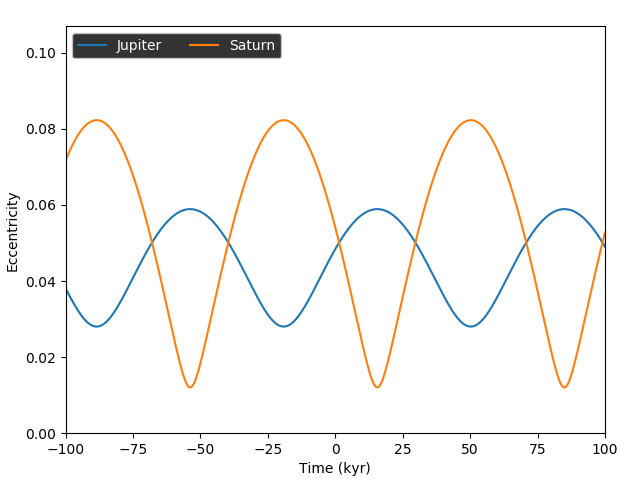
\includegraphics[width=\textwidth]{JS_ecc.png}
       	 \caption{Evolution of eccentricity of Jupiter and Saturn.}
        	\label{}
    \end{subfigure}
    \begin{subfigure}[t]{0.49\textwidth}
    %\captionsetup{justification=centering}
    \captionsetup{width=0.9\textwidth}
        	\centering
	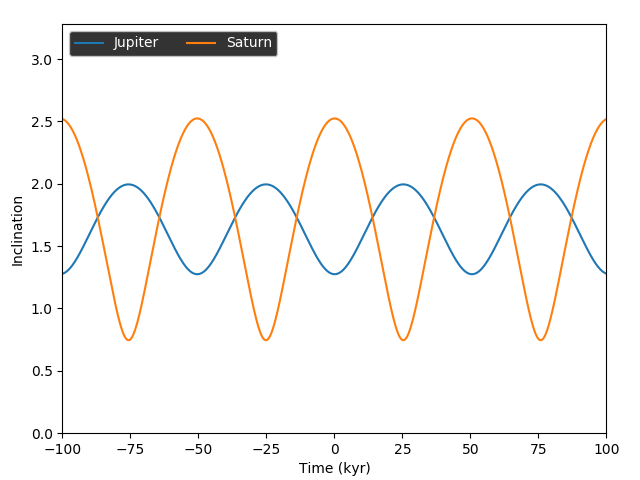
\includegraphics[width=\textwidth]{JS_inc.png}
        	\caption{Evolution of inclination of Jupiter and Saturn.}
        	\label{}
    \end{subfigure}
    \caption{}
    \label{JSout}
\end{figure}

\textbf{Verdict}: Figure \ref{JSout} is a very good match to that of the output in Murray \& Dermott (1999)\cite{ssd}.

\subsubsection{Whole Solar System}

The plots for the eccentricity and inclination of each planet are as shown:
\begin{figure}[!h]
    \centering
    \begin{subfigure}[t]{0.49\textwidth}
    %\captionsetup{justification=centering}
    \captionsetup{width=0.9\textwidth}
	\centering
       	 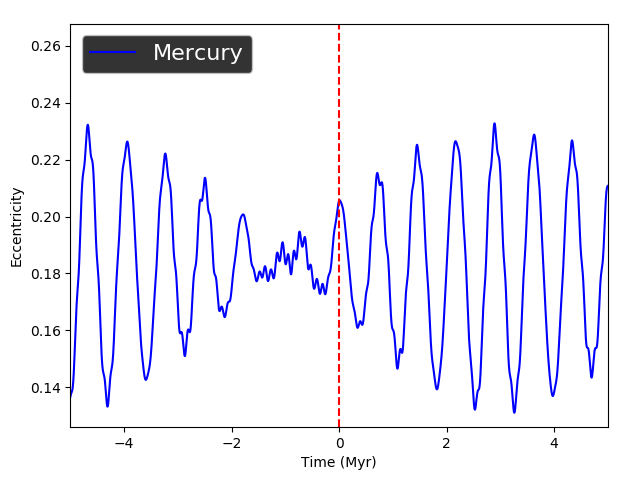
\includegraphics[width=\textwidth]{Eccentricity_Mercury}
    \end{subfigure}
    \begin{subfigure}[t]{0.49\textwidth}
    %\captionsetup{justification=centering}
    \captionsetup{width=0.9\textwidth}
        	\centering
	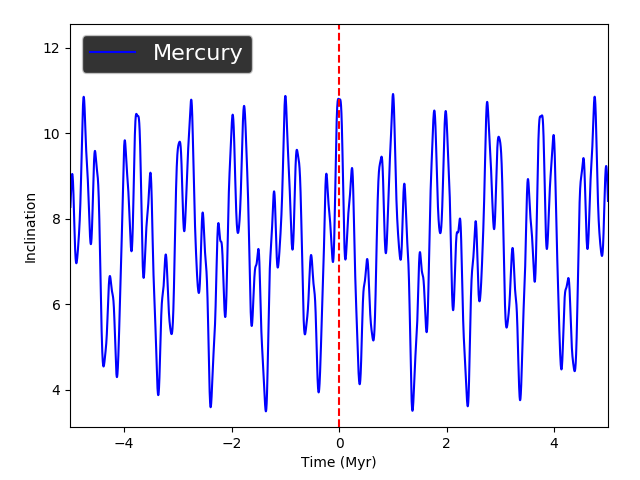
\includegraphics[width=\textwidth]{Inclination_Mercury}
    \end{subfigure}
\end{figure}
\begin{figure}[!h]
	\ContinuedFloat
    \centering
    \begin{subfigure}[t]{0.49\textwidth}
    %\captionsetup{justification=centering}
    \captionsetup{width=0.9\textwidth}
	\centering
       	 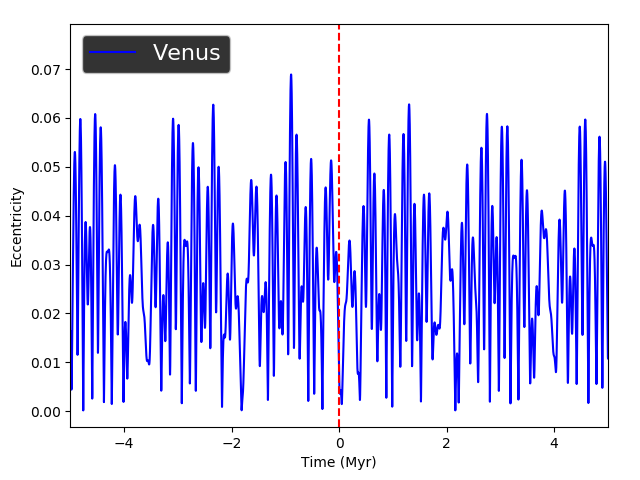
\includegraphics[width=\textwidth]{Eccentricity_Venus}
    \end{subfigure}
    \begin{subfigure}[t]{0.49\textwidth}
    %\captionsetup{justification=centering}
    \captionsetup{width=0.9\textwidth}
        	\centering
	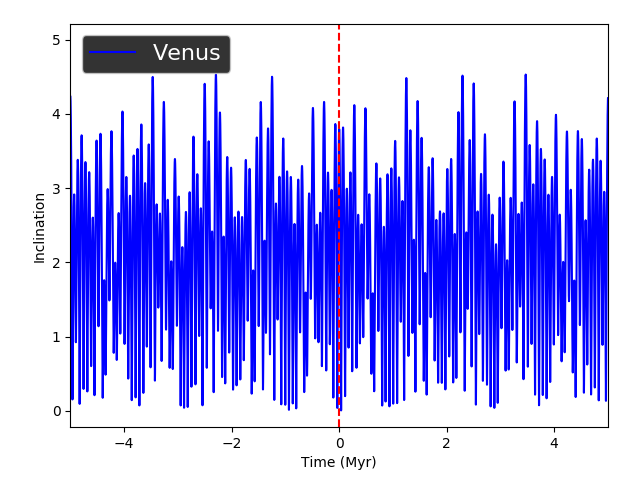
\includegraphics[width=\textwidth]{Inclination_Venus}
    \end{subfigure}
\end{figure}
\begin{figure}[!h]
	\ContinuedFloat
    \centering
    \begin{subfigure}[t]{0.49\textwidth}
    %\captionsetup{justification=centering}
    \captionsetup{width=0.9\textwidth}
	\centering
       	 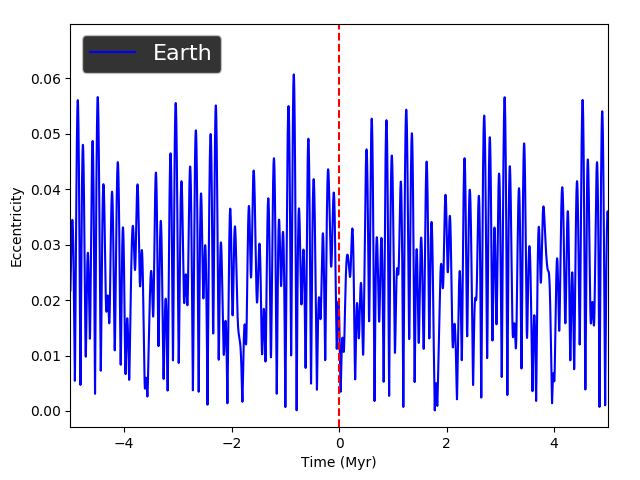
\includegraphics[width=\textwidth]{Eccentricity_Earth}
    \end{subfigure}
    \begin{subfigure}[t]{0.49\textwidth}
    %\captionsetup{justification=centering}
    \captionsetup{width=0.9\textwidth}
        	\centering
	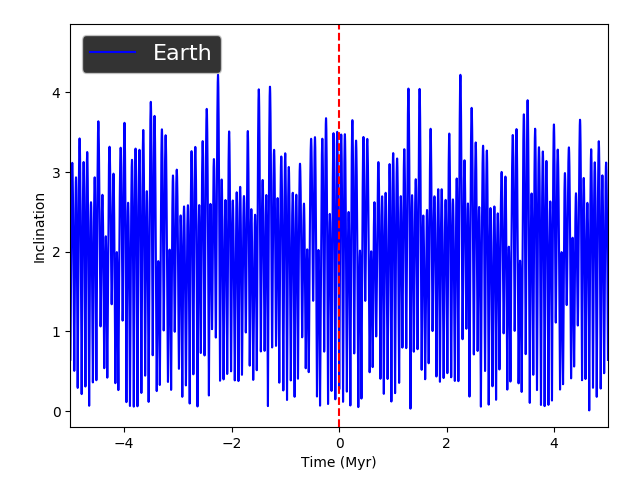
\includegraphics[width=\textwidth]{Inclination_Earth}
    \end{subfigure}
\end{figure}
\begin{figure}[!h]
	\ContinuedFloat
    \centering
    \begin{subfigure}[t]{0.49\textwidth}
    %\captionsetup{justification=centering}
    \captionsetup{width=0.9\textwidth}
	\centering
       	 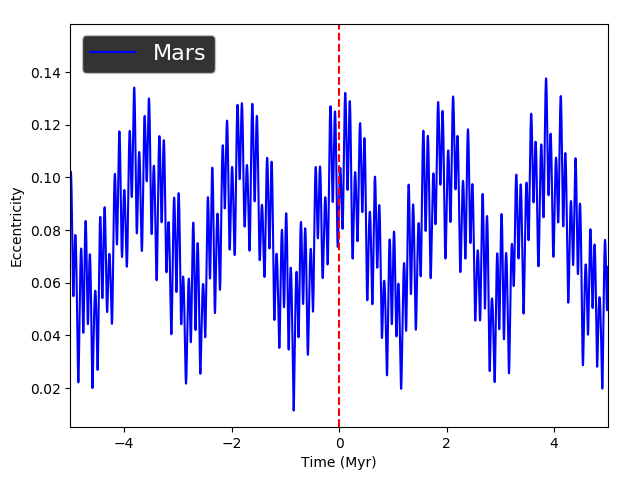
\includegraphics[width=\textwidth]{Eccentricity_Mars}
    \end{subfigure}
    \begin{subfigure}[t]{0.49\textwidth}
    %\captionsetup{justification=centering}
    \captionsetup{width=0.9\textwidth}
        	\centering
	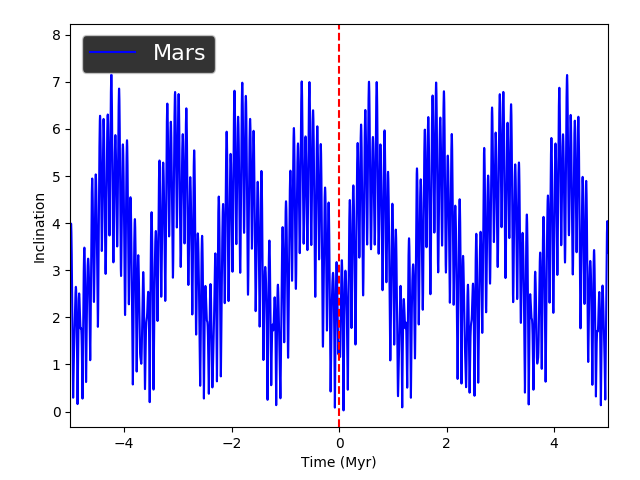
\includegraphics[width=\textwidth]{Inclination_Mars}
    \end{subfigure}
\end{figure}
\begin{figure}[!h]
	\ContinuedFloat
    \centering
    \begin{subfigure}[t]{0.49\textwidth}
    %\captionsetup{justification=centering}
    \captionsetup{width=0.9\textwidth}
	\centering
       	 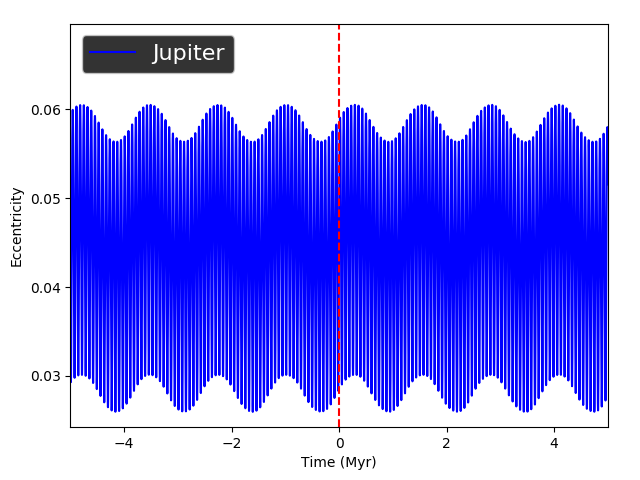
\includegraphics[width=\textwidth]{Eccentricity_Jupiter}
    \end{subfigure}
    \begin{subfigure}[t]{0.49\textwidth}
    %\captionsetup{justification=centering}
    \captionsetup{width=0.9\textwidth}
        	\centering
	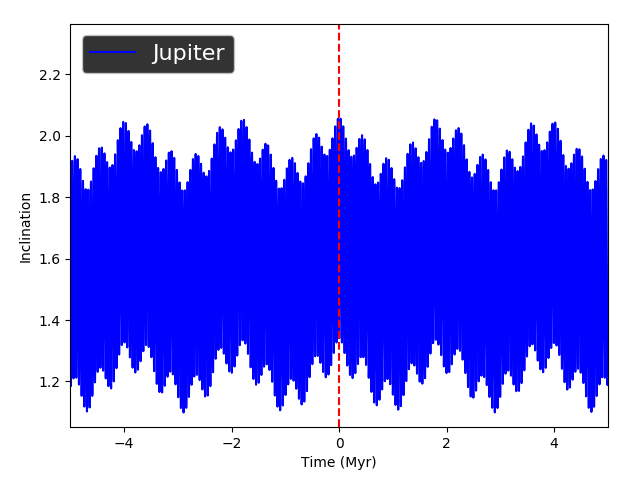
\includegraphics[width=\textwidth]{Inclination_Jupiter}
    \end{subfigure}
\end{figure}
\begin{figure}[!h]
	\ContinuedFloat
    \centering
    \begin{subfigure}[t]{0.49\textwidth}
    %\captionsetup{justification=centering}
    \captionsetup{width=0.9\textwidth}
	\centering
       	 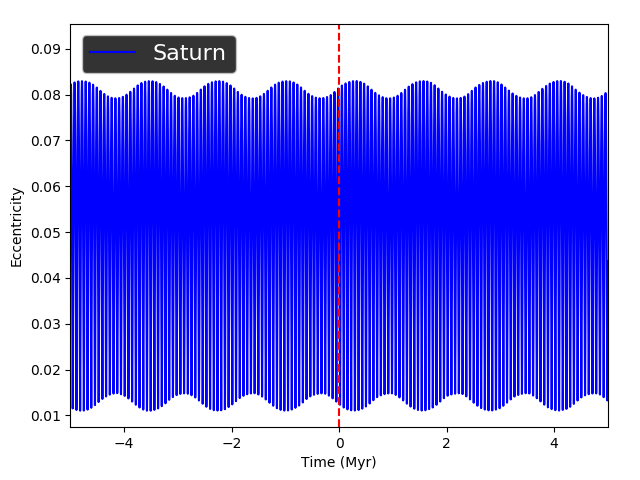
\includegraphics[width=\textwidth]{Eccentricity_Saturn}
    \end{subfigure}
    \begin{subfigure}[t]{0.49\textwidth}
    %\captionsetup{justification=centering}
    \captionsetup{width=0.9\textwidth}
        	\centering
	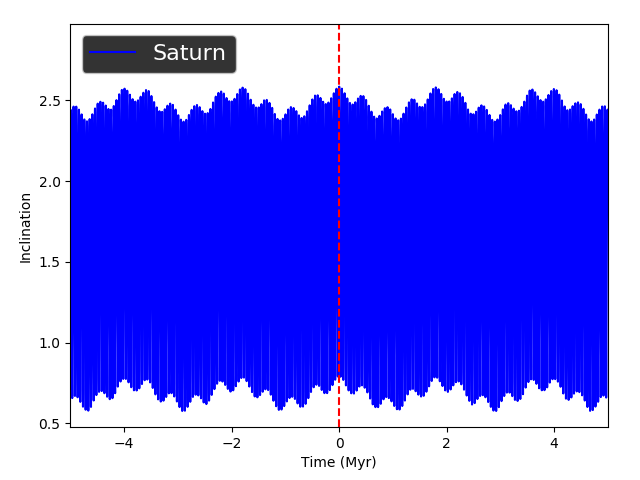
\includegraphics[width=\textwidth]{Inclination_Saturn}
    \end{subfigure}
\end{figure}
\begin{figure}[!h]
	\ContinuedFloat
    \centering
    \begin{subfigure}[t]{0.49\textwidth}
    %\captionsetup{justification=centering}
    \captionsetup{width=0.9\textwidth}
	\centering
       	 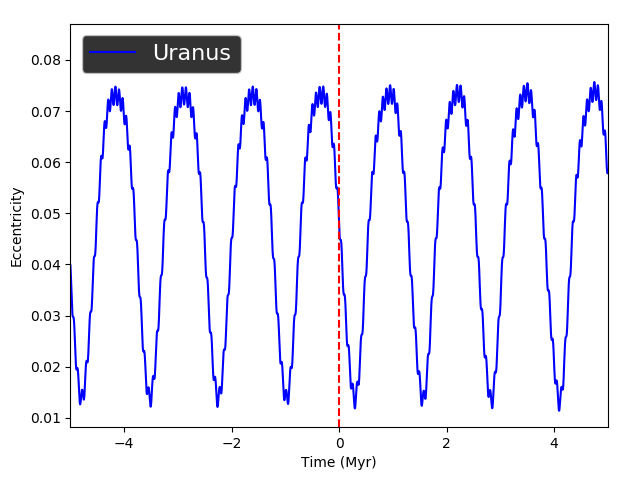
\includegraphics[width=\textwidth]{Eccentricity_Uranus}
    \end{subfigure}
    \begin{subfigure}[t]{0.49\textwidth}
    %\captionsetup{justification=centering}
    \captionsetup{width=0.9\textwidth}
        	\centering
	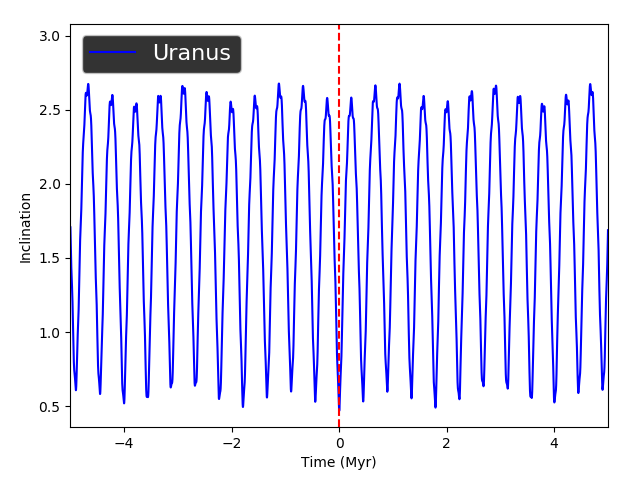
\includegraphics[width=\textwidth]{Inclination_Uranus}
    \end{subfigure}
\end{figure}
\begin{figure}[!h]
	\ContinuedFloat
    \centering
    \begin{subfigure}[t]{0.49\textwidth}
    %\captionsetup{justification=centering}
    \captionsetup{width=0.9\textwidth}
	\centering
       	 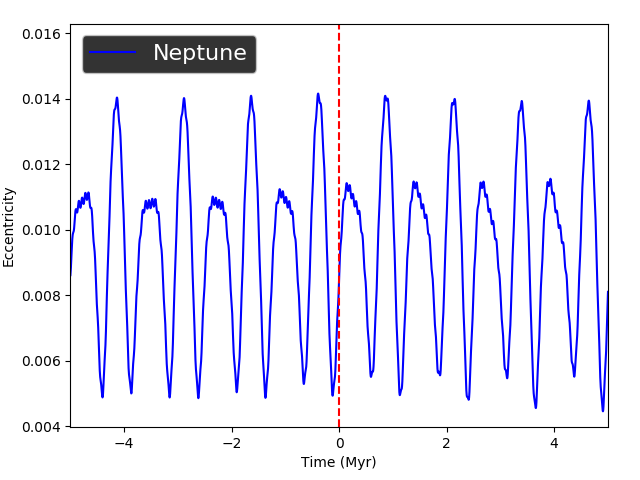
\includegraphics[width=\textwidth]{Eccentricity_Neptune}
    \end{subfigure}
    \begin{subfigure}[t]{0.49\textwidth}
    %\captionsetup{justification=centering}
    \captionsetup{width=0.9\textwidth}
        	\centering
	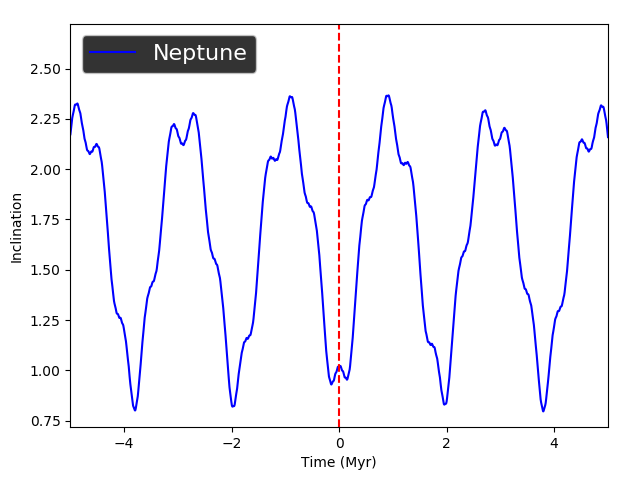
\includegraphics[width=\textwidth]{Inclination_Neptune}
    \end{subfigure}
    \caption{Eccentricity and inclination (in degrees) of each planet in the Solar System using J2000 data.}
\end{figure}

\newpage
\ 
\newpage
\
\newpage

\subsubsection*{Verdict}

By comparing these plots with existing results \cite{ssd, texas}, it can be seen that the results are consistent with what is expected. It should be noted that the eccentricity plots do not match with Murray \& Dermott as well as the inclinations. However when comparing the max and min eccentricity (especially Mercury) to the other data\cite{texas}, the eccentricities do match well. Oddly, the inclinations in the other data\cite{texas} do not match as well; has lower $I_{min}$ and higher $I_{max}$.

\subsubsection{Precession of mercury}

Another test that serves as a good indicator of the accuracy of the simulation is determining the precession of Mercury. Applying Laplace-Lagrange secular theory is expected to yield a precession rate, $\dot{\varpi}$ of $544{}'' yr^{-1}$\cite{texas, PRMer}.

\subsubsection*{Verdict}

From Figure \ref{fig:pidot}, it can be seen the mean precession, the red dashed line is equal to $544.86{}''$ per century; consistent with expectations and without the addition of General Relativity. The plot of the precession rate also matched with expected results\cite{texas}.

The effect of the oblateness of the Sun on the precession rate of Mercury was also found to be $\sim 0.08{}''$ per century. The small magnitude of the change is as expected.
        
\begin{figure}[!h]
    \centering
    \begin{subfigure}[t]{0.49\textwidth}
    %\captionsetup{justification=centering}
    \captionsetup{width=0.9\textwidth}
	\centering
       	 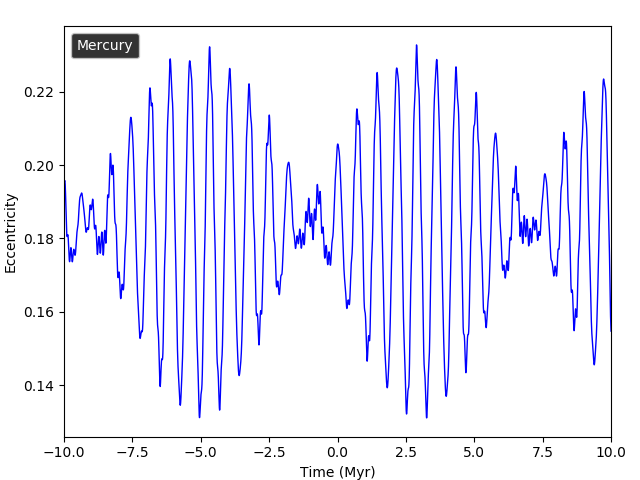
\includegraphics[width=\textwidth]{Merc_ecc.png}
       	 \caption{Evolution of eccentricity of Mercury.}
        	\label{}
    \end{subfigure}
    \begin{subfigure}[t]{0.49\textwidth}
    %\captionsetup{justification=centering}
    \captionsetup{width=0.9\textwidth}
        	\centering
	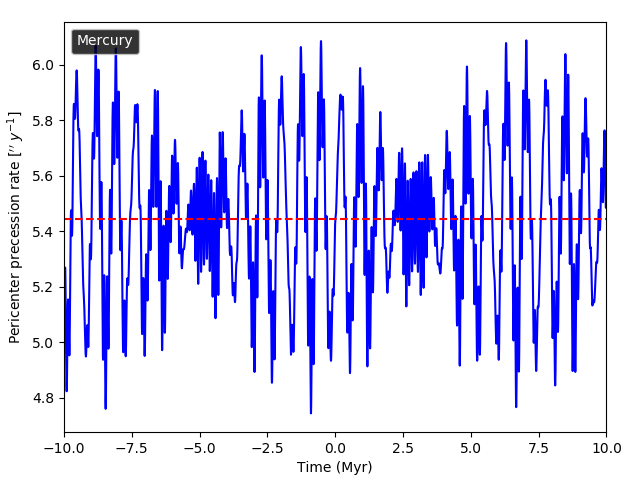
\includegraphics[width=\textwidth]{Merc_pidot.png}
        	\caption{Precession rate, $\dot{\varpi}$ of Mercury.}
        	\label{fig:pidot}
    \end{subfigure}
    \caption{}
    \label{Merc1}
\end{figure}

\newpage
\
\newpage

\section{October 1$^{st} - $8$^{th}$ 2017}

\subsection{Keplerian to Cartesian coordinates}

The next test to check accuracy is to convert the output of the equations of motion to cartesian coordinates in order to plot the Solar System for visual inspection. For this we use:
\begin{itemize}
\item $h, k, p, q$ - the equations of motion.
\item $e$ - the eccentricity.
\item $i$ - the inclination (in radians).
\item $a$ - the semi-major axis (in $AU$).
\item $n$ - the orbital frequency (in radians per year)
\end{itemize}
First the mean anomaly, $M(t)$ is found using
\begin{equation}
M(t) = n(t-t_{0}).
\end{equation}
Then the eccentric anomaly $E \equiv E(t)$ is calculated by solving
\begin{equation}
M(t) = E(t) - e\sin E(t)
\end{equation}
using the Newton-Raphson method:
\begin{equation}
E_{j+1} = E_{j} - \frac{f(E_{j})}{\frac{d}{dE_{j}}f(E_{j})} = E_{j} - \frac{E_{j} - e\sin E_{j} - M}{1-e\cos E_{j}}, \hspace*{1cm} E_{0}=M
\end{equation}
The above equation was iterated until $E_{j+1} = E_{j}$. Then the true anomaly $\nu(t)$ was calculated using
\begin{equation}
\nu(t) = 2 \, \text{arctan2} \left (\sqrt{1+e} \sin \frac{E(t)}{2}, \sqrt{1-e} \cos \frac{E(t)}{2} \right).
\end{equation}
Where $ \text{arctan2}$ is the two argument arctangent function. The distance $r_{c}$ from the central body was then calculated using
\begin{equation}
r_{c} = a(1-e \cos E(t)).
\end{equation}
Then the position vector in the orbital frame was found using
\begin{equation}
\mathbf{o}(t) = \begin{pmatrix}
o_{x}(t)\\ 
o_{y}(t)\\ 
o_{z}(t)
\end{pmatrix} = r_{c}(t) \begin{pmatrix}
\cos \nu(t)\\ 
\sin \nu(t)\\ 
0
\end{pmatrix}
\end{equation}
Then $\Omega$, the longitude of the ascending node, and $\omega$, the argument of the periapsis was found using
\begin{subequations}
   \begin{equation}
   \Omega =  \text{arctan2}(p, q),
   \end{equation}
   \begin{equation}
   \omega = \Omega - \text{arctan2}(h, k).
   \end{equation}
\end{subequations}
Finally the cartesian coordinates could be found using
\begin{equation}
\mathbf{r}(t) = \begin{pmatrix}
o_{x}(t)(\cos(\omega)\cos(\Omega)-\sin(\omega)\cos(i)\sin(\Omega))-o_{y}(t)(\sin(\omega)\cos(\Omega)+\cos(\omega)\cos(i)\sin(\Omega))\\ 
o_{x}(t)(\cos(\omega)\sin(\Omega)+\sin(\omega)\cos(i)\cos(\Omega))+o_{y}(t)(\cos(\omega)\cos(i)\cos(\Omega)-\sin(\omega)\sin(\Omega))\\ 
o_{x}(t)(\sin(\omega)\sin(i))+o_{y}(t)(\cos(\omega)\sin(i))
\end{pmatrix}
\end{equation}


\textbf{Code}:
\begin{lstlisting}[language=Python, caption={Converting from Keplerian to Cartesian coordinates}]
    def get_pi_or_omega(self, hp, kq):
        pi_om = []
        for i in range(len(self.planets)):
            pi_om.append(np.arctan2(hp[i], kq[i]))
        return np.array(pi_om)

    def kep2cart(self, ecc, inc, h_list, k_list, p_list, q_list, time, t0, idx):
        O_list = self.get_pi_or_omega(p_list, q_list)
        w_list = O_list-self.get_pi_or_omega(h_list, k_list)
        n = self.get_property_all_planets('n')
        a = self.get_property_all_planets('a')

        Mt = n[idx]*np.pi/180*(time-t0)
        EA = []
        e, w, O, i = ecc[idx], w_list[idx], O_list[idx], inc[idx]
        for t in range(len(time)):
            E = Mt[t]
            f_by_dfdE = (E-e[t]*np.sin(E)-Mt[t])/(1-e[t]*np.cos(E))
            j, maxIter, delta = 0, 30, 0.0000000001
            while (j < maxIter)*(np.abs(f_by_dfdE) > delta):
                E = E-f_by_dfdE
                f_by_dfdE = (E-e[t]*np.sin(E)-Mt[t])/(1-e[t]*np.cos(E))
                j += 1
            EA.append(E)
        EA = np.array(EA)
        nu = 2*np.arctan2(np.sqrt(1+e)*np.sin(EA/2), np.sqrt(1-e)*np.cos(EA/2))

        rc = a[idx]*(1-e*np.cos(EA))
        o_vec = np.array([rc*np.cos(nu), rc*np.sin(nu), 0])

        rx = (o_vec[0]*(np.cos(w)*np.cos(O) - np.sin(w)*np.cos(i)*np.sin(O)) - o_vec[1]*(np.sin(w)*np.cos(O) + np.cos(w)*np.cos(i)*np.sin(O)))
        ry = (o_vec[0]*(np.cos(w)*np.sin(O) + np.sin(w)*np.cos(i)*np.cos(O)) + o_vec[1]*(np.cos(w)*np.cos(i)*np.cos(O) - np.sin(w)*np.sin(O)))
        rz = (o_vec[0]*(np.sin(w)*np.sin(i)) + o_vec[1]*(np.cos(w)*np.sin(i)))

        return rx, ry, rz
\end{lstlisting}

\subsection{Test of conversion}

To test the conversion and the accuracy of the simulation, the Solar System was simulated for 1000 years and plotted below in Cartesian coordinates.

\begin{figure}[!h]
\begin{center}
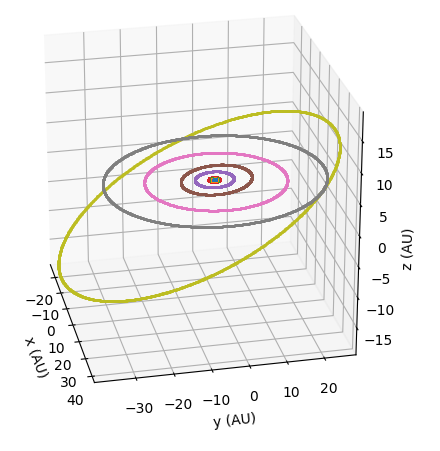
\includegraphics[width= 0.8\textwidth]{SolarSystem3D_rsz}
\caption[]{Plot of the Solar System simulated for a 1000 years from J2000 data.}
\label{}
\end{center}
\end{figure}

\textbf{Verdict}: The plot is as expected. The plot was also used to ensure the time period of orbits were as expected, which they were.

\subsection{General Relativity corrections}

General Relativity (GR) corrections add an additional term to $\dot{\varpi}_{j}$. This additional term is given by \cite{Adams2006}
\begin{equation}
\dot{\varpi}_{j}^{GR} = 3\frac{a_{j}^{2}n_{j}^{3}}{c^{2}}.
\end{equation}
This term is added to the diagonal elements of $\mathbf{A}$ to accounts for the effects of GR.

\subsection{Test of GR correction}
\label{GRcor}

To test the effects of GR on the precession rates $\dot{\varpi}$, each planet was simulated by itself and its precession rate was calculated. The effect of GR on $\dot{\varpi}$, in arc seconds per century, of each planet is shown below

\begin{verbatim}
Mercury : 42.8928
Venus : 8.6069 
Earth : 3.8309
Mars : 1.3483 
Jupiter : 0.0621 
Saturn : 0.0137 
Uranus : 0.0024 
Neptune : 0.0008 
Pluto : 0.0004 
\end{verbatim}

The inclusion of GR had the largest effect on Mercury, as expected. This can be seen in the difference of the eccentricity plots in Figure \ref{Merc2} and previously in Figure \ref{Merc1}.

\begin{figure}[!h]
    \centering
    \begin{subfigure}[t]{0.49\textwidth}
    %\captionsetup{justification=centering}
    \captionsetup{width=0.9\textwidth}
	\centering
       	 \includegraphics[width=\textwidth]{Mercury_ecc_GR.png}
       	 \caption{Evolution of eccentricity of Mercury.}
        	\label{}
    \end{subfigure}
    \begin{subfigure}[t]{0.49\textwidth}
    %\captionsetup{justification=centering}
    \captionsetup{width=0.9\textwidth}
        	\centering
	\includegraphics[width=\textwidth]{Mercury_pidot_GR.png}
        	\caption{Precession rate, $\dot{\varpi}$ of Mercury.}
        	\label{fig:pidot}
    \end{subfigure}
    \caption{Effect of GR on the orbit of Mercury.}
    \label{Merc2}
\end{figure}

\textbf{Verdict}: These values match very well to calculated values of GR's affect \cite{GRpidot}. Additionally, including the effect of GR has also resulted in the eccentricity plot of Mercury becoming a closer match to Murray \& Dermott (1999) \cite{ssd}.

\newpage

\section{October 9$^{th} - $15$^{th}$ 2017}

\subsection{Eccentricity damping corrections}

We assume that the tides raised by planets are more dominant relative to tides raised by the star. Thus the eccentricity damping rate is given by \cite{ssd, Zhang2013}
\begin{equation}
\lambda = -\frac{\dot{e}}{e} = \frac{63}{4} \frac{1}{Q{}'_{p}}\frac{m_{\star}}{m_{p}} \left (\frac{R_{p}}{a_{p}} \right)^{5} n_{p}.
\end{equation}
Where $R$ is the radius of the planet, $Q{}' \equiv 1.5Q/k_{2}$ is the modified tidal quality factor. $Q$ is the tidal quality factor and $k_{2}$ is the Love number of degree 2 of the planet. All other terms are the same as before. The values of $Q$ and $k_{2}$ are taken from Goldreich \& Sotter (1966)\cite{Goldreich1966}, Zhang (1992)\cite{Zhang1992}, and Gavrilov \& Kharkov (1977)\cite{Gavrilov1977}. Similarly to the GR correction, $\sqrt{-1}\lambda$ is added to diagonal elements of $\mathbf{A}$ to account for the effect of tides.

Since the correction involved complex numbers, the code had to be adapted to work with complex numbers as opposed to real numbers. To do this, all data containers now store \texttt{dtype=`complex128'}. The only major change involved altering Code \ref{solveS_Phase} for solving for the scale factors and phase and is outline below.
\begin{lstlisting}[language=Python, caption={Change to Code \ref{solveS_Phase}}]
def f(x, *boundaries):
    s_factor, phase = x
    return [s_factor*np.sin(phase)-boundaries[0], s_factor*np.cos(phase)-boundaries[1]]

def real_scaling_factor_and_phase(x1, *boundaries):
    s_factor, phase = x1[0]+1j*x1[1], x1[2]+1j*x1[3] 
    x = [s_factor, phase]
    actual_f = f(x, *boundaries)
    return [np.real(actual_f[0]), np.imag(actual_f[0]), np.real(actual_f[1]), np.imag(actual_f[1])]
\end{lstlisting}

\subsection{Test of eccentricity damping}

As before with GR, the effect of eccentricity damping is tested on the precession rate of the planets. It was found that this additional had no effect, at least on timescales of a few million years. However, for the Solar System, only a small change is expected, on timescales of billions of years.

\subsection{Animating the Solar System}

To be able to perform quick visual tests of the simulation (a few years at a time), code was written to create an animation of the solar system.

\begin{lstlisting}[language=Python, caption={Animating the Solar System}]
mport numpy as np
import pylab
import glob
import os
from matplotlib import pyplot as plt
from mpl_toolkits.mplot3d import Axes3D
import matplotlib.animation
import pandas as pd

files = glob.glob('Animate_solar_system/*.csv')
files.sort(key=os.path.getmtime)
files = "\n".join(files).split('\n')

n_planets = 4
colours = ['r', 'orange', 'b', 'g', 'brown', 'r', 'orange', 'b', 'g']

fig = plt.figure()
ax = fig.add_subplot(111, projection='3d')
ttl = ax.text(0, 1.05, 0, 'Time = years', transform = ax.transAxes, va='center')

all_x, all_y, all_z = [], [], []
points = []
for idx in range(n_planets):
    points.append(None)
    
    df = pd.read_csv(files[idx])
    x, y, z = np.array(df.x), np.array(df.y), np.array(df.z)
    all_x.append(x)
    all_y.append(y)
    all_z.append(z)
xyz = np.array([all_x, all_y, all_z])

def update_graph(num):
    global points
    global ttl
    data=df

    for idx in range(n_planets):
        if points[idx] is not None:
            points[idx].set_color(colours[idx])
            points[idx].set_markersize(1)
        points[idx], = ax.plot(all_x[idx][num:num+1], all_y[idx][num:num+1], all_z[idx][num:num+1], linestyle="", marker="o", color=colours[idx])
    ttl.set_text('Time = {:.2f} years'.format(df.time[num]))
    if num%5 == 0 and num > 10:
        if num%25 == 0:
            plt.cla()
            ttl = ax.text(0, 1.05, 0, '', transform = ax.transAxes, va='center')
            ax.plot(x0, y0, z0, 'b*', markersize=3, zorder=-999)
            ax.set_zlabel('z (AU)')
            ax.set_xlabel('x (AU)')
            ax.set_ylabel('y (AU)')
        
        ttl.set_text('Time = {:.2f} years'.format(df.time[num]))
        for idx in range(n_planets):
            ax.plot(all_x[idx][:num-1], all_y[idx][:num-1], all_z[idx][:num-1], linestyle="", marker="o", color=colours[idx], markersize=1)
            max_axis = np.max([np.abs(np.min(xyz)), np.max(xyz)])
            ax.set_zlim(-max_axis, max_axis)
            ax.set_ylim(-max_axis, max_axis)
            ax.set_xlim(-max_axis, max_axis)
    return graph, 

x0, y0, z0 = np.zeros(2), np.zeros(2), np.zeros(2)
graph, = ax.plot(x0, y0, z0, 'b*', markersize=3, zorder=-999)

ax.view_init(45, 45)
max_axis = np.max([np.abs(np.min(xyz)), np.max(xyz)])
ax.set_zlim(-max_axis, max_axis)
ax.set_ylim(-max_axis, max_axis)
ax.set_xlim(-max_axis, max_axis)
ax.set_zlabel('z (AU)')
ax.set_xlabel('x (AU)')
ax.set_ylabel('y (AU)')

ani = matplotlib.animation.FuncAnimation(fig, update_graph, len(x), 
                               interval=1, save_count=50, repeat=False) 
ani.save('Animate_solar_system/Plots/rocky_planets.mp4', fps=24)
\end{lstlisting}

After viewing the animation it was found that all the planets behaved normally with 1 exception; Earth. The behaves normally at all times $t < 0$ years. However during $0 \leq t \leq 1$ years, the Earth behaves in an unexpected manner, at $t > 1$ years, the behaviour of the Earth returns to normal.  This behaviour is also only seen if both Venus and Jupiter are present in the simulation.

The cause of this bug is unknown for now. However it does not have any effect on long term simulations (as seen by results in \S\ref{GRcor}) due to the very short duration of the bug. Hence, the simulation can now be tested on other star systems.

\subsection{Simulating other planet systems}

\subsubsection{Extracting data}


The data of other star systems were taken from \href{https://exoplanetarchive.ipac.caltech.edu/}{Nasa Exoplanet Archive}. To aid in the extraction of data, a web crawler that takes the star alias as the argument was written.

\begin{lstlisting}[language=Python, caption={Extracting data from \href{https://exoplanetarchive.ipac.caltech.edu/}{Nasa Exoplanet Archive}}]
import glob
import os
import sys
from bs4 import BeautifulSoup
from unidecode import unidecode
import requests
import numpy as np
import pandas as pd
from scipy import stats
import numpy.ma as ma

def mean_data(obj_id):
	'''''
	Extracts the mean data of each planet in the star system.
	'''''
    obj_id_split = obj_id.split(' ')
    obj_id = obj_id_split[0]
    output_id = obj_id_split[0]
    for i in range(1, len(obj_id_split)):
        obj_id += '+'+obj_id_split[i]
        output_id += '_'+obj_id_split[i]

    url = "https://exoplanetarchive.ipac.caltech.edu/cgi-bin/ExoOverview/nph-ExoOverview?objname={}&type=&label&aliases&exo&iden&orb&ppar&tran&note&disc&ospar&ts&nalc&force=&dhxr1507830887922".format(obj_id)
    response = requests.get(url)

    bs = BeautifulSoup(response.content, "html.parser")

    for idx, title in enumerate(bs.findAll('div', {'class': 'data'})):
        name = title.find('th').text
        if name == 'Planet Orbital Properties':
            index = idx

    planet_props = bs.findAll('div', {'class': 'data'})

    column_names = []
    planets = []
    p_idx = 0

    for idx, text in enumerate(planet_props[index].findAll()):
        text = unidecode(str(text))

        if 'th' in text:
            if 'class' not in text:
                if 'Reference' not in text:
                    if 'href' not in text:
                        column_names.append(text[4:-5])

        if idx > 1:
            text_split = text.split('\n')
            for t in text_split:
                if 'td' in t:
                    if 'href' not in t:
                        t = t[4:-5]
                        if '+-' in t:
                            t = t.split('+-')[0].split(' ')[-1]
                            planets[p_idx-1].append(t)
                        elif 'lt' in t or 'gt' in t:
                            t = t.split(';')[-1]
                            planets[p_idx-1].append(t)
                        else:
                            t = t.split('span')
                            if len(t) == 1:
                                t = t[0].split(' ')[-1]
                                if 'null' not in t:
                                    if t.isdigit() or '.' in t:
                                        planets[p_idx-1].append(t)
                                    else:
                                        if len(t) == 1:
                                            planets.append([])
                                            planets[p_idx].append(t)
                                            p_idx += 1
                                else:
                                    planets[p_idx-1].append(t)
                            else:
                                t = t[1].split('>')[1].split('<')[0]
                                planets[p_idx-1].append(t)
    planets = planets[::2]

    column_names_2 = []
    planets_2 = []
    p_idx = 0

    for idx, title in enumerate(bs.findAll('div', {'class': 'data'})):
        name = title.find('th').text
        if name == 'Planet Parameters':
            index = idx

    found_highlight = False
    for idx, text in enumerate(planet_props[index].findAll()):
        text = unidecode(str(text))

        if 'th' in text:
            if 'tr' not in text:
                if 'class' not in text:
                    if 'span' not in text:
                        if '(' in text:
                            t = text[5:-6]
                            if 'sup' in t:
                                t = t.split('<')[0]
                            column_names_2.append(t)
                            
        if idx > 1:
            text_split = text.split('\n')
            for t in text_split:
                if 'td' in t:
                    if 'href' not in t:
                        t = t[4:-5]
                        if '+-' in t:
                            t = t.split('+-')[0].split(' ')[-1]
                            planets_2[p_idx-1].append(t)
                        elif 'lt' in t or 'gt' in t:
                            t = t.split(';')[-1]
                            planets_2[p_idx-1].append(t)
                        else:
                            t = t.split('span')
                            if len(t) == 1:
                                t = t[0].split(' ')[-1]
                                if 'null' not in t:
                                    if t.isdigit() or '.' in t:
                                        planets_2[p_idx-1].append(t)
                                    else:
                                        if len(t) == 1:
                                            planets_2.append([])
                                            # planets_2[p_idx].append(t)
                                            p_idx += 1
                                else:
                                    if len(t) == 1:
                                        planets_2[p_idx-1].append(t)
                                    elif 'null' in t:
                                        planets_2[p_idx-1].append(t)
                            else:
                                t = t[1].split('>')[1].split('<')[0]
                                planets_2[p_idx-1].append(t)

    planets_2 = planets_2[::2]

    for i in range(len(planets)):
        planets[i].extend(planets_2[i])
    
    for i in column_names_2:
        column_names.append(i)
   
    column_names = np.array(column_names)
    for c, col in enumerate(column_names):
        if col == 'Planet':
            column_names[c] = 'Name'
        if col == 'Period (days)':
            column_names[c] = 'n'
        if col == 'Semi-Major Axis (AU)':
            column_names[c] = 'a'
        if col == 'Inclination (deg)':
            column_names[c] = 'i'
        if col == 'Eccentricity':
            column_names[c] = 'e'
        if col == 'Longitude of Periastron (deg)':
            column_names[c] = 'pi'
        if col == 'Earth Mass':
            column_names[c] = 'Mass'
        if col == 'Jupiter Mass':
            column_names[c] = 'Mj'

    mass_idx = np.where(['Mass' in x for x in column_names])[0]
    column_names[mass_idx[-1]] = 'Mass_2'

    planets = np.array(planets)

    labels, n_data = np.unique(planets[:, 0], return_counts=True)
    start_idx = np.zeros_like(labels)
    for s, l in enumerate(labels):
        start_idx[s] = np.where(planets[:, 0] == l)[0][0]
    start_idx = np.array(start_idx, dtype='int')

    planet_means = []

    for l in range(len(labels)):
        planet_means.append([])
        planet_means[l].append(labels[l])
        for col in range(1, planets.shape[1]):
            col_data = planets[:, col][start_idx[l]:start_idx[l]+n_data[l]]
            planet_l_data = ma.masked_array(col_data, col_data == 'null').compressed()
            try:
                compressed_array = ma.array(planet_l_data, dtype=float)
                if len(compressed_array) > 0:
                    planet_means[l].append(ma.mean(compressed_array))
                else:
                    planet_means[l].append(np.nan)
            except:
                print('null')
    
    planet_means = np.array(planet_means)

    columns_to_ignore = ['Passage', 'Date', 'Mj', 'Radii', 'g/cm', 'K']
    idxs = []
    for word in columns_to_ignore:
        idx = np.where([word in x for x in column_names])[0]
        for i in idx:
            idxs.append(i)

    df = pd.DataFrame(columns=column_names, index=range(0, len(planet_means)))
    for row in range(len(planet_means)):
        for col in range(len(column_names)):
            df.ix[row, col] = planet_means[row, col]
            if planet_means[row, col] == 'null':
                df.ix[row, col] = np.nan
            if col in idxs:
                df.ix[row, col] = np.nan
    
    return df

def read_data(obj_id):
	''''''
	Extracts the data from the highlighted row of each planet in the star system.
	''''''
    obj_id_split = obj_id.split(' ')
    obj_id = obj_id_split[0]
    output_id = obj_id_split[0]
    for i in range(1, len(obj_id_split)):
        obj_id += '+'+obj_id_split[i]
        output_id += '_'+obj_id_split[i]

    url = "https://exoplanetarchive.ipac.caltech.edu/cgi-bin/ExoOverview/nph-ExoOverview?objname={}&type=&label&aliases&exo&iden&orb&ppar&tran&note&disc&ospar&ts&nalc&force=&dhxr1507830887922".format(obj_id)
    print('\nExtracting data of {} from:\n{}\n'.format(output_id, url))
    response = requests.get(url)

    bs = BeautifulSoup(response.content, "html.parser")

    for idx, title in enumerate(bs.findAll('div', {'class': 'data'})):
        name = title.find('th').text
        if name == 'Planet Orbital Properties':
            index = idx
            # print(name, idx)

    planet_props = bs.findAll('div', {'class': 'data'})

    planets = []
    column_names = []
    p_idx = 0

    found_highlight = False
    for idx, text in enumerate(planet_props[index].findAll()):
        text = unidecode(str(text))

        found_highlight = 'class="overview_highlight"' in text
        if 'th' in text:
            if 'class' not in text:
                if 'Reference' not in text:
                    if 'href' not in text:
                        column_names.append(text[4:-5])
                        
        if idx > 1:
            if found_highlight:
                text_split = text.split('\n')
                for t in text_split:
                    if 'tr' not in t:
                        if 'href' not in t:
                            t = t[4:-5]
                            if '+-' in t:
                                t = t.split('+-')[0].split(' ')[-1]
                                planets[p_idx-1].append(t)
                            elif 'lt' in t or 'gt' in t:
                                t = t.split(';')[-1]
                                planets[p_idx-1].append(t)
                            else:
                                t = t.split('span')
                                if len(t) == 1:
                                    t = t[0].split(' ')[-1]
                                    if 'null' not in t:
                                        if t.isdigit() or '.' in t:
                                            planets[p_idx-1].append(t)
                                        else:
                                            planets.append([])
                                            planets[p_idx].append(t)
                                            p_idx += 1
                                    else:
                                        planets[p_idx-1].append(t)
                                else:
                                    t = t[1].split('>')[1].split('<')[0]
                                    planets[p_idx-1].append(t)
            found_highlight=False

    p_idx = 0

    for idx, title in enumerate(bs.findAll('div', {'class': 'data'})):
        name = title.find('th').text
        if name == 'Planet Parameters':
            index = idx

    found_highlight = False
    for idx, text in enumerate(planet_props[index].findAll()):
        text = unidecode(str(text))

        found_highlight = 'class="overview_highlight"' in text
        if 'th' in text:
            if 'tr' not in text:
                if 'class' not in text:
                    if 'span' not in text:
                        if '(' in text:
                            t = text[5:-6]
                            if 'sup' in t:
                                t = t.split('<')[0]
                            column_names.append(t)
                            
        if idx > 1:
            if found_highlight:
                text_split = text.split('\n')
                for t in text_split:
                    try:
                        if 'tr' not in t:
                            if 'href' not in t:
                                t = t[4:-5]
                                if '+-' in t:
                                    t = t.split('+-')[0].split(' ')[-1]
                                    planets[p_idx-1].append(t)
                                elif 'lt' in t or 'gt' in t:
                                    t = t.split(';')[-1]
                                    planets[p_idx-1].append(t)
                                else:
                                    t = t.split('span')
                                    if len(t) == 1:
                                        t = t[0].split(' ')[-1]
                                        if 'null' not in t:
                                            if t.isdigit() or '.' in t:
                                                planets[p_idx-1].append(t)
                                            else:
                                                p_idx += 1
                                        else:
                                            planets[p_idx-1].append(t)
                                    else:
                                        t = t[1].split('>')[1].split('<')[0]
                                        # print(p_idx, end=', ')
                                        planets[p_idx-1].append(t)
                    except:
                        print(t)
            found_highlight=False

    column_names = column_names[:]
    column_names = np.array(column_names)
    for c, col in enumerate(column_names):
        if col == 'Planet':
            column_names[c] = 'Name'
        if col == 'Period (days)':
            column_names[c] = 'n'
        if col == 'Semi-Major Axis (AU)':
            column_names[c] = 'a'
        if col == 'Inclination (deg)':
            column_names[c] = 'i'
        if col == 'Eccentricity':
            column_names[c] = 'e'
        if col == 'Longitude of Periastron (deg)':
            column_names[c] = 'pi'
        if col == 'Earth Mass':
            column_names[c] = 'Mass'
        if col == 'Jupiter Mass':
            column_names[c] = 'Mj'

    mass_idx = np.where(['Mass' in x for x in column_names])[0]
    column_names[mass_idx[-1]] = 'Mass_2'

    planets = np.array(planets)

    columns_to_ignore = ['Passage', 'Date', 'Mj', 'Radii', 'g/cm', 'K']
    idxs = []
    for word in columns_to_ignore:
        idx = np.where([word in x for x in column_names])[0]
        for i in idx:
            idxs.append(i)

    df = pd.DataFrame(columns=column_names, index=range(0, np.shape(planets)[0]))
    for row in range(np.shape(planets)[0]):
        for col in range(np.shape(planets)[1]):
            df.ix[row, col] = planets[row, col]
            if planets[row, col] == 'null':
                df.ix[row, col] = np.nan
            if col in idxs:
                df.ix[row, col] = np.nan

    for idx, title in enumerate(bs.findAll('div', {'class': 'data'})):
        name = title.find('th').text
        if name == 'Summary of Stellar Information':
            index = idx

    star_prop = []
    found_highlight = False
    for idx, text in enumerate(planet_props[index].findAll()):
        text = unidecode(str(text))

        found_highlight = 'Mass' in text
        if idx > 1:
            if found_highlight:
                text_split = text.split('\n')
                for t in text_split:
                    if 'tr' not in t:
                        if 'null' not in t:
                            if 'class' not in t:
                                t = t[4:-5].split('+-')
                                star_prop.append(float(t[0]))
                found_highlight = False
                
    df1 = pd.DataFrame(columns=['star_mass', 'star_radius'], index=range(0, 1))
    df1.ix[0, 0] = star_prop[0]
    if len(star_prop) == 1:
        df1.ix[0, 1] = np.nan
    else:
        df1.ix[0, 1] = star_prop[1]

    return df, df1

def compare_data(df_highlighted, df_average, output_id):
    rows, cols = df_highlighted.shape

    mass_idx = df_highlighted.columns.get_loc("Mass")
    n_idx = df_highlighted.columns.get_loc("n")
    for row in range(rows):
        for col in range(cols):
            if pd.isnull(df_highlighted.ix[row, col]) and not pd.isnull(df_average.ix[row, col]):
                df_highlighted.ix[row, col] = df_average.ix[row, col]

            if col == mass_idx:
                if str(df_highlighted.ix[row, col+2]) != 'nan':
                    df_highlighted.ix[row, col] = df_highlighted.ix[row, col+2]
            if col == n_idx:
                df_highlighted.ix[row, col] = 2*np.pi/(float(df_highlighted.ix[row, col])/365)*180/np.pi
    
    cols_to_keep = ['Name', 'n', 'a', 'e', 'i', 'pi', 'Mass']
    for pi in df_highlighted['pi']:
        if pi == 'nan':
            print('WARNING: nans exist for values of pi')
            break
    df_highlighted[cols_to_keep].to_csv('Exoplanets_data/'+output_id+'/'+'planets.csv', index=False)

if __name__ == '__main__':
    # obj_id = '55 Cnc'

    if len(sys.argv) > 1:
        obj_id = sys.argv[1]
        args = sys.argv[2:]
        for a in args:
            obj_id += ' '+a
        obj_id = list(obj_id)
        for index, s in enumerate(obj_id):
            if s == '+':
                obj_id[index] = '%2B'
        obj_id = "".join(obj_id)

    df_highlight, df_star = read_data(obj_id)
    df_mean = mean_data(obj_id)

    obj_id_split = obj_id.split(' ')
    output_id = obj_id_split[0]
    for i in range(1, len(obj_id_split)):
        output_id += '_'+obj_id_split[i]

    folder = glob.glob('Exoplanets_data/'+output_id)
    if len(folder) == 0:
        os.system('mkdir '+'Exoplanets_data/'+output_id)

    compare_data(df_highlight, df_mean, output_id)
    df_star.to_csv('Exoplanets_data/'+output_id+'/'+'star.csv', index=False)

\end{lstlisting}

To use the code, either uncomment line 432 and replace the string with star id to extract data from, or in the terminal type: \texttt{python planet\_data\_crawler\_v2.py <star\_id>}.

\subsubsection{Simulation results}


\begin{longtable}{|l|c|c|c|c|c|c|c|}
\caption{Eccentricity results of various star systems}
\label{my-label} \\
\hline
\rowcolor[HTML]{C0C0C0} 
Planet  & $m \ (M_{\oplus})$ & $a \ (AU)$ & $e_{obs}$ & $\bar{e}$ & $\sigma_{e}$ & $e_{max}$ & $e_{min}$ \\ \hline
\endfirsthead
\multicolumn{8}{c}%
{{\bfseries \tablename\ \thetable{} -- continued from previous page}} \\
\hline
\rowcolor[HTML]{C0C0C0} 
Planet  & $m \ (M_{\oplus})$ & $a$ & $e_{obs}$ & $\bar{e}$ & $\sigma_{e}$ & $e_{max}$ & $e_{min}$ \\ \hline\endhead
\hline \multicolumn{8}{|r|}{{Continued on next page}} \\ \hline
\endfoot

\endlastfoot

\hline
24 Sex b      & 632.46  & 1.333 & 0.090   & 0.129   & 0.039  & 0.179  & 0.067  \\ 
24 Sex c      & 273.32  & 2.080 & 0.290   & 0.254   & 0.036  & 0.301  & 0.200  \\ \hline
61 Vir b      & 5.10    & 0.050 & 0.120   & 0.202   & 0.045  & 0.284  & 0.114  \\ 
61 Vir c      & 18.20   & 0.218 & 0.140   & 0.232   & 0.072  & 0.335  & 0.113  \\ 
61 Vir d      & 22.90   & 0.476 & 0.350   & 0.314   & 0.030  & 0.355  & 0.266  \\ \hline
BD+20 2457 b  & 6807.63 & 1.450 & 0.150   & 0.140   & 0.058  & 0.211  & 0.039  \\ 
BD+20 2457 c  & 3963.17 & 2.010 & 0.180   & 0.161   & 0.076  & 0.251  & 0.010  \\ \hline
CoRoT-7 b     & 5.74    & 0.017 & 0.000   & 0.000   & 0.000  & 0.000  & 0.000  \\ 
CoRoT-7 c     & 8.40    & 0.046 & 0.000   & 0.000   & 0.000  & 0.000  & 0.000  \\ \hline
GJ 163 b      & 10.60   & 0.061 & 0.073   & 0.081   & 0.013  & 0.100  & 0.060  \\ 
GJ 163 c      & 6.80    & 0.125 & 0.099   & 0.090   & 0.013  & 0.109  & 0.069  \\ 
GJ 163 d      & 29.40   & 1.030 & 0.373   & 0.373   & 0.000  & 0.373  & 0.373  \\ \hline
GJ 876 b      & 635.63  & 0.208 & 0.032   & 0.071   & 0.025  & 0.104  & 0.027  \\ 
GJ 876 c      & 177.98  & 0.130 & 0.256   & 0.203   & 0.037  & 0.256  & 0.143  \\ 
GJ 876 d      & 6.03    & 0.021 & 0.207   & 0.190   & 0.012  & 0.207  & 0.172  \\ 
GJ 876 e      & 14.60   & 0.334 & 0.055   & 0.134   & 0.043  & 0.199  & 0.054  \\ \hline
HAT-P-13 b    & 270.46  & 0.043 & 0.013   & 0.010   & 0.005  & 0.016  & 0.001  \\ 
HAT-P-13 c    & 4538.42 & 1.223 & 0.662   & 0.662   & 0.000  & 0.662  & 0.662  \\ \hline
HD 11964 b    & 198.00  & 3.160 & 0.041   & 0.041   & 0.001  & 0.041  & 0.040  \\ 
HD 11964 c    & 25.00   & 0.229 & 0.300   & 0.300   & 0.000  & 0.300  & 0.300  \\ \hline
HD 12661 b    & 691.57  & 0.808 & 0.377   & 0.309   & 0.052  & 0.377  & 0.230  \\ 
HD 12661 c    & 575.88  & 2.815 & 0.031   & 0.156   & 0.071  & 0.241  & 0.028  \\ \hline
HD 128311 b   & 562.20  & 1.084 & 0.303   & 0.212   & 0.103  & 0.334  & 0.004  \\ 
HD 128311 c   & 993.20  & 1.740 & 0.159   & 0.198   & 0.045  & 0.257  & 0.129  \\ \hline
HD 133131 A b & 451.00  & 1.440 & 0.330   & 0.332   & 0.097  & 0.457  & 0.174  \\ 
HD 133131 A c & 133.00  & 4.490 & 0.490   & 0.448   & 0.139  & 0.626  & 0.218  \\ \hline
HD 134987 b   & 505.00  & 0.810 & 0.233   & 0.229   & 0.002  & 0.233  & 0.226  \\ 
HD 134987 c   & 260.00  & 5.800 & 0.120   & 0.125   & 0.003  & 0.129  & 0.120  \\ \hline
HD 142 b      & 397.27  & 1.020 & 0.170   & 0.165   & 0.031  & 0.208  & 0.122  \\ 
HD 142 c      & 1684.40 & 6.800 & 0.210   & 0.210   & 0.002  & 0.213  & 0.207  \\ \hline
HD 160691 b   & 343.24  & 1.497 & 0.128   & 0.084   & 0.031  & 0.129  & 0.025  \\ 
HD 160691 c   & 576.52  & 5.235 & 0.099   & 0.100   & 0.002  & 0.103  & 0.098  \\ 
HD 160691 d   & 10.55   & 0.091 & 0.172   & 0.170   & 0.002  & 0.174  & 0.167  \\ 
HD 160691 e   & 165.87  & 0.921 & 0.067   & 0.146   & 0.046  & 0.210  & 0.065  \\ \hline
HD 190360 b   & 495.79  & 4.010 & 0.313   & 0.313   & 0.000  & 0.313  & 0.313  \\ 
HD 190360 c   & 19.07   & 0.130 & 0.237   & 0.235   & 0.001  & 0.237  & 0.234  \\ \hline
HD 202206 b   & 5530.00 & 0.830 & 0.435   & 0.416   & 0.026  & 0.452  & 0.379  \\ 
HD 202206 c   & 776.00  & 2.550 & 0.267   & 0.340   & 0.139  & 0.509  & 0.095  \\ \hline
HD 217107 b   & 441.77  & 0.075 & 0.127   & 0.127   & 0.000  & 0.127  & 0.127  \\ 
HD 217107 c   & 826.32  & 5.320 & 0.517   & 0.517   & 0.000  & 0.517  & 0.517  \\ \hline
HD 3167 b     & 5.02    & 0.018 & 0.000   & 0.024   & 0.010  & 0.041  & 0.000  \\ 
HD 3167 c     & 9.80    & 0.180 & 0.267   & 0.316   & 0.033  & 0.362  & 0.267  \\ 
HD 3167 d     & 6.90    & 0.078 & 0.360   & 0.232   & 0.106  & 0.360  & 0.033  \\ \hline
HD 37124 b    & 215.00  & 0.534 & 0.054   & 0.145   & 0.070  & 0.245  & 0.023  \\ 
HD 37124 c    & 207.00  & 1.710 & 0.125   & 0.113   & 0.050  & 0.192  & 0.002  \\ 
HD 37124 d    & 221.00  & 2.807 & 0.160   & 0.120   & 0.041  & 0.191  & 0.026  \\ \hline
HD 38529 b    & 266.65  & 0.131 & 0.257   & 0.254   & 0.004  & 0.262  & 0.249  \\ 
HD 38529 c    & 4252.39 & 3.712 & 0.341   & 0.341   & 0.000  & 0.341  & 0.341  \\ \hline
HD 73526 b    & 715.09  & 0.650 & 0.290   & 0.263   & 0.049  & 0.329  & 0.188  \\ 
HD 73526 c    & 715.09  & 1.030 & 0.280   & 0.312   & 0.142  & 0.483  & 0.047  \\ \hline
HD 74156 b    & 572.07  & 0.292 & 0.627   & 0.631   & 0.026  & 0.662  & 0.583  \\ 
HD 74156 c    & 2561.60 & 3.850 & 0.432   & 0.432   & 0.002  & 0.436  & 0.429  \\ \hline
HD 80606 b    & 1252.20 & 0.449 & 0.933   & 0.933   & 0.000  & 0.933  & 0.933  \\ \hline
Kepler-30 b   & 11.30   & 0.180 & 0.042   & 0.034   & 0.006  & 0.043  & 0.025  \\ 
Kepler-30 c   & 640.00  & 0.300 & 0.011   & 0.011   & 0.001  & 0.012  & 0.009  \\ 
Kepler-30 d   & 23.10   & 0.500 & 0.022   & 0.027   & 0.006  & 0.034  & 0.018  \\ \hline
ups And b     & 218.53  & 0.059 & 0.022   & 0.022   & 0.000  & 0.022  & 0.021  \\ 
ups And c     & 629.60  & 0.828 & 0.260   & 0.269   & 0.008  & 0.280  & 0.258  \\ 
ups And d     & 1313.22 & 2.513 & 0.299   & 0.206   & 0.081  & 0.306  & 0.067  \\ \hline
\end{longtable}



\begin{figure}[!h]
\begin{center}
\includegraphics[width= \textwidth]{exoplanet_eccs}
\caption[]{}
\label{}
\end{center}
\end{figure}

\newpage

\section{October 16$^{th} - $22$^{nd}$ 2017}

 
\newpage

\titleformat{\section}{\normalfont\large\bfseries}{\thesection}{1em}{}
\let\oldaddcontentsline\addcontentsline% Store \addcontentsline
\renewcommand{\addcontentsline}[3]{}% Make \addcontentsline a no-op

\bibliography{LogbookBib} 
\bibliographystyle{ieeetr}

\let\addcontentsline\oldaddcontentsline% Restore \addcontentsline
\end{document}
